\documentclass[11pt]{article}

% ---- Packages ---------------------------------------------------------------
\usepackage[margin=1in]{geometry}
\usepackage{amsmath,amssymb,amsthm}
\usepackage{graphicx}
\usepackage{subcaption}
\usepackage[colorlinks=true,linkcolor=blue!60!black,citecolor=blue!60!black,urlcolor=blue!60!black]{hyperref}
\usepackage[round,sort,comma]{natbib}
\usepackage{booktabs}
\usepackage{algorithm}
\usepackage{algpseudocode}
\usepackage{xcolor}
\usepackage{setspace}
\usepackage{caption}
\usepackage[textsize=small]{todonotes}

% ---- Figure paths -----------------------------------------------------------
% Local compilation:  figures are in the same directory as main.tex,
%                     model schematics are one level up in tutorials/
% Overleaf:           copy avecilla_wf_model.png, chuong_wf_model.png,
%                     de_et_al_model.png, zhou_model.png from tutorials/
%                     into the Overleaf project root and change the second
%                     path below to {./}
\graphicspath{{./}{../tutorials/}}

% ---- Convenient macros ------------------------------------------------------
\newcommand{\btheta}{\boldsymbol{\theta}}
\newcommand{\bx}{\mathbf{x}}
\newcommand{\E}{\mathbb{E}}
\newcommand{\R}{\mathbb{R}}

% ---- Document ---------------------------------------------------------------
\begin{document}

\title{\textbf{Simulation-Based Inference for Experimental Evolution:\\
Prior Sensitivity, Ensembles, and Model Misspecification}}

\author{[Author list placeholder]}

\date{}
\maketitle

\begin{abstract}
Simulation-based inference~(SBI) has become an attractive approach for
experimental evolution because stochastic population-genetic simulators are
easy to write while likelihoods are often analytically intractable.
Yet the practical reliability of SBI in this setting remains underexplored:
posterior estimates can depend strongly on the prior, neural estimators may
vary across training runs, and model misspecification can yield confident but
misleading inferences.

Here we study these issues using copy-number-variant~(CNV) and aneuploidy
dynamics in \emph{Saccharomyces cerevisiae} as testbeds.
Across a family of Wright-Fisher and chemostat-based simulators, we compare
approximate Bayesian computation~(ABC) with neural SBI methods, and use both
synthetic and empirical datasets to identify when inference is stable and
when it becomes fragile.
Three findings motivate the paper.
First, posterior concentration in realistic evolutionary datasets can be
strongly prior-sensitive, particularly when trajectories are short and noisy.
Second, ensemble-based inference provides a practical route to more stable
posterior estimation than a single trained neural posterior.
Third, applying even a closely related but biologically incorrect simulator
produces systematic posterior-predictive mismatch, showing that model
checking is not optional in this domain.

The paper therefore serves two purposes.
It introduces a reusable SBI workflow for experimental evolution, and it
uses that workflow to make a research argument about reliability:
good inference depends not only on the choice of algorithm, but also on
prior design, model adequacy, and estimator stability.
Jupyter notebooks accompanying the manuscript provide the executable
supplement.
\end{abstract}

\tableofcontents

% =============================================================================
\section{Introduction}
\label{sec:intro}
% =============================================================================

Experimental evolution---the controlled propagation of microbial or cellular
populations under defined selective conditions---has become one of the most
powerful tools in evolutionary biology
\citep{lenski2017experimental,barrick2013genome}.
Laboratory evolution experiments allow researchers to observe evolutionary
change in real time, with population sizes, environmental conditions, and
genetic compositions measured at every passage.
A particularly tractable system is the unicellular yeast \emph{Saccharomyces
cerevisiae}, which can be propagated in chemostats or serial batch cultures
for hundreds of generations while fluorescent reporters track the frequency of
specific genetic variants.

A central quantitative goal in such experiments is \emph{parameter
inference}: given a time-series of variant frequencies, what are the
underlying mutation rate, selection coefficient, and initial frequency of the
variant?
These three quantities jointly determine the pace and repeatability of
adaptive evolution, yet none of them is directly observable.
Answering this question with classical statistical tools is frustrated by the
stochastic nature of population dynamics.
The Wright-Fisher model \citep{ewens2004mathematical}, the workhorse of
theoretical population genetics, accurately captures the combined effects of
genetic drift, selection, and mutation, but its likelihood function has no
closed-form expression for the multi-timepoint frequency trajectories that
experiments produce.
This makes gradient-based or conjugate Bayesian methods inapplicable.

Simulation-based inference (SBI) \citep{cranmer2020frontier} resolves this
impasse.
Rather than evaluating the likelihood analytically, SBI generates a large
library of~$({\btheta}, \bx)$ pairs by forward simulation, then uses this
library to either select parameter values whose simulations closely match the
observed data (Approximate Bayesian Computation, ABC) or to train a neural
network to approximate the posterior density directly (Neural Posterior
Estimation, NPE, and related methods).
SBI has been applied across a broad range of scientific domains including
neuroscience, cosmology, and epidemiology
\citep{cranmer2020frontier,lueckmann2021benchmarking}, and was first applied
to experimental evolution by \citet{avecilla2022neural}.

Despite the recent success of SBI in biology, three practical questions
remain central for experimental evolution.
How much of the inferred posterior is driven by the data versus the prior?
How stable is a neural posterior estimator across repeated training runs?
And how badly does inference fail when the simulator is only slightly wrong?
These are especially important in evolutionary systems, where datasets are
often short, replicate counts are modest, and mechanistic misspecification is
easy to introduce.

\subsection{Research Question and Scope}

The central goal of this paper is to study the practical reliability of SBI
for experimental-evolution data.
We do so in a deliberately mechanistic setting: we work with small,
interpretable population-genetic simulators, and we ask how inference
behaves when one varies the prior, the inference estimator, or the simulator
class itself.

This manuscript is therefore not meant as a general review of SBI.
Instead, it uses a focused collection of evolutionary systems to make a
research argument about three related issues: prior sensitivity, ensemble
stabilisation, and model misspecification.
These questions are methodological, but they also matter biologically,
because they determine whether inferred mutation rates and selection
coefficients can be trusted.

\subsection{Main Findings and Paper Roadmap}

The paper has three main findings:
\begin{enumerate}
  \item \textbf{Prior sensitivity matters.}
        In realistic inference regimes, posterior concentration can depend
        strongly on prior support and prior shape, particularly for mutation
        rates and low-frequency founder states.
  \item \textbf{Ensembles improve stability.}
        Repeated neural posterior estimators need not agree exactly even when
        trained on the same simulator family; ensemble-based inference offers
        a practical way to reduce estimator variance and improve robustness.
  \item \textbf{Model misspecification is easy to diagnose if one looks for
        it.}
        Applying the wrong simulator, even from a closely related
        experimental system, produces systematic posterior-predictive
        mismatch and can lead to misleading biological conclusions.
\end{enumerate}

To support these claims, the paper proceeds in three layers.
Sections~\ref{sec:problem} and \ref{sec:simulators} define the inference
problem and the simulator family.
Section~\ref{sec:sbi} summarises the SBI methods under comparison.
Section~\ref{sec:applications} then uses synthetic and empirical systems to
show where the workflow succeeds, where it is prior-sensitive, and where it
fails under misspecification.

For completeness, we also include a short section on the collective
posterior for combining evidence across replicates
(Section~\ref{sec:collective}).
That topic is part of a separate companion methods paper and is included here
mainly because multi-replicate experiments are standard in this field.

% =============================================================================
\section{The Inference Problem in Experimental Evolution}
\label{sec:problem}
% =============================================================================

\subsection{Experimental setup and data structure}

A typical experimental evolution dataset consists of $r$ independent
replicate populations, each observed at $T$ discrete time points
$t_1 < t_2 < \cdots < t_T$ (measured in generations or passages).
At each time point the frequency $x_{i,t} \in [0,1]$ of one or more genetic
variants is measured, often via flow cytometry of fluorescent reporters.
The complete dataset for replicate~$i$ is the trajectory
$\bx_i = (x_{i,t_1},\ldots,x_{i,t_T}) \in [0,1]^T$.

Our goal is to infer the parameter vector $\btheta$ that governs the
evolutionary dynamics.
Depending on the biological question, $\btheta$ typically includes some
combination of:
\begin{itemize}
  \item $s$ --- selection coefficient (fitness advantage per generation),
  \item $\delta$ or $m$ --- de~novo mutation or copy-number-change rate per
        cell division,
  \item $\phi$ or $p_0$ --- initial frequency of the variant, and
  \item population-size-related parameters (sometimes fixed from independent
        measurements).
\end{itemize}

A key feature of experimental evolution is \emph{stochasticity at multiple
levels}.
Even with identical underlying parameters, two replicate trajectories will
differ because of:
(i) \emph{genetic drift}---the multinomial sampling noise inherent to
finite-population evolution, and
(ii) \emph{between-replicate parameter variation}---subtle differences in
actual mutation rates, initial frequencies, or effective population sizes.
Any inference framework must account for both sources of variation.

\subsection{Why standard methods fail}

For a Wright-Fisher model with multiple genotypes and time points, the
likelihood $p(\bx \mid \btheta)$ is a product of multinomial transition
probabilities integrated over all possible intermediate population states.
This integral is analytically intractable for more than two time points or
more than two alleles in a finite population \citep{tataru2017statistical}.
Diffusion approximations exist in limiting cases but break down when drift is
strong (small $N$) or mutation rates are high.
Maximum-likelihood methods therefore require either restrictive model
simplifications or approximate numerical schemes that do not generalise across
model classes.

SBI takes a different approach: instead of computing the likelihood, it uses
the simulator itself as an implicit model, and learns the posterior from
simulated data.

% =============================================================================
\section{Stochastic Population-Genetic Simulators}
\label{sec:simulators}
% =============================================================================

\subsection{The Wright-Fisher model}
\label{sec:wf}

The Wright-Fisher (WF) model describes the evolution of a finite population
of $N$ haploid individuals with $K$ distinct genotypes.
Let $\mathbf{c}_t = (c_{1,t},\ldots,c_{K,t})$ denote the counts of each
genotype at generation~$t$, with $\sum_k c_{k,t} = N$.
One generation of evolution proceeds in two steps:
\begin{enumerate}
  \item \textbf{Selection.} Compute the fitness-weighted frequency of each
        genotype:
        \begin{equation}
          f_{k,t} = \frac{w_k \, c_{k,t}}{\sum_{j=1}^{K} w_j \, c_{j,t}},
          \label{eq:selection}
        \end{equation}
        where $w_k$ is the (relative) fitness of genotype $k$.
  \item \textbf{Drift.} Sample the next-generation counts multinomially:
        \begin{equation}
          \mathbf{c}_{t+1} \sim \mathrm{Multinomial}(N,\, \mathbf{f}_t).
          \label{eq:drift}
        \end{equation}
\end{enumerate}
Mutation is incorporated by modifying $\mathbf{f}_t$ before sampling, using
a transition matrix $M$ whose entry $M_{jk}$ is the probability that a copy
of genotype $k$ produces a copy of genotype $j$ in one generation.

All simulators in this tutorial share this basic structure; they differ in
the number of genotypes, the form of the transition matrix, and whether
fitness is a fixed parameter or derived from an underlying ODE model.
The simulator is computationally cheap (milliseconds per trajectory) and
can be parallelised trivially, making it ideal for the large simulation
budgets that SBI requires.

\subsection{Modelling copy-number variants}
\label{sec:cnv_models}

Copy-number variants (CNVs) arise when a chromosomal segment is duplicated or
deleted, producing multi-copy or zero-copy configurations of a gene.
In nitrogen-limited chemostat or batch evolution experiments with
\emph{S. cerevisiae}, amplifications of nutrient-transporter genes (e.g.,
\emph{GAP1}) recurrently confer a selective advantage, making CNV frequency a
tractable observable for parameter inference.

We work with three distinct CNV models, each designed for a different
experimental context (Figures~\ref{fig:model_schematics}a--c).

\paragraph{Four-genotype batch model (Chuong et al.).}
This model was developed for batch evolution experiments in which populations
are propagated by discrete serial dilution \citep{chuong2025template}.
The four genotypes are: (i) wild-type~(WT), (ii) CNV\textsuperscript{+}
(cells carrying an amplification), (iii) CNV\textsuperscript{$-$} (cells
that transiently carry a pre-existing, copy-neutral CNV precursor), and
(iv) SNV (point-mutant competitors).
The parameter vector is
$\btheta = (\log s,\, \log \delta,\, \log \phi)$, where $s$ is the CNV
selection coefficient, $\delta$ is the de~novo CNV formation rate per cell
division, and $\phi$ is the initial frequency of CNV\textsuperscript{$-$}
cells.
The model runs for $T=12$ discrete time points (generations 8--116) with
$N = 10^7$ (effective population size in batch culture).

\paragraph{Three-genotype chemostat model (Avecilla et al.).}
This model, introduced by \citet{avecilla2022neural}, captures continuous
chemostat evolution with three genotypes: ancestor ($X_A$), CNV beneficial
mutation ($X_C$), and other beneficial mutation~($X_B$).
The parameter vector is
$\btheta = (\log\delta_C,\, \log\delta_B,\, s_C,\, s_B)$, where subscripts
$C$ and $B$ refer to CNV and other beneficial mutations respectively.
The effective population size is $N = 3.3\times10^8$.

\paragraph{Two-genotype reversion model (De et al.).}
CNVs that confer a fitness advantage under selection may revert to single copy
upon removal of selection pressure \citep{de2025segmental}.
This model tracks CNV\textsuperscript{+} cells reverting to a diploid
ancestor, with parameters
$\btheta = (\log s,\, \log m,\, \log p_0)$, where $s$ is the fitness cost of
the CNV in non-selective media, $m$ is the reversion rate, and $p_0$ is the
initial CNV frequency.
The effective population size is $N = 1.9\times10^6$.

\begin{figure}[ht]
  \centering
  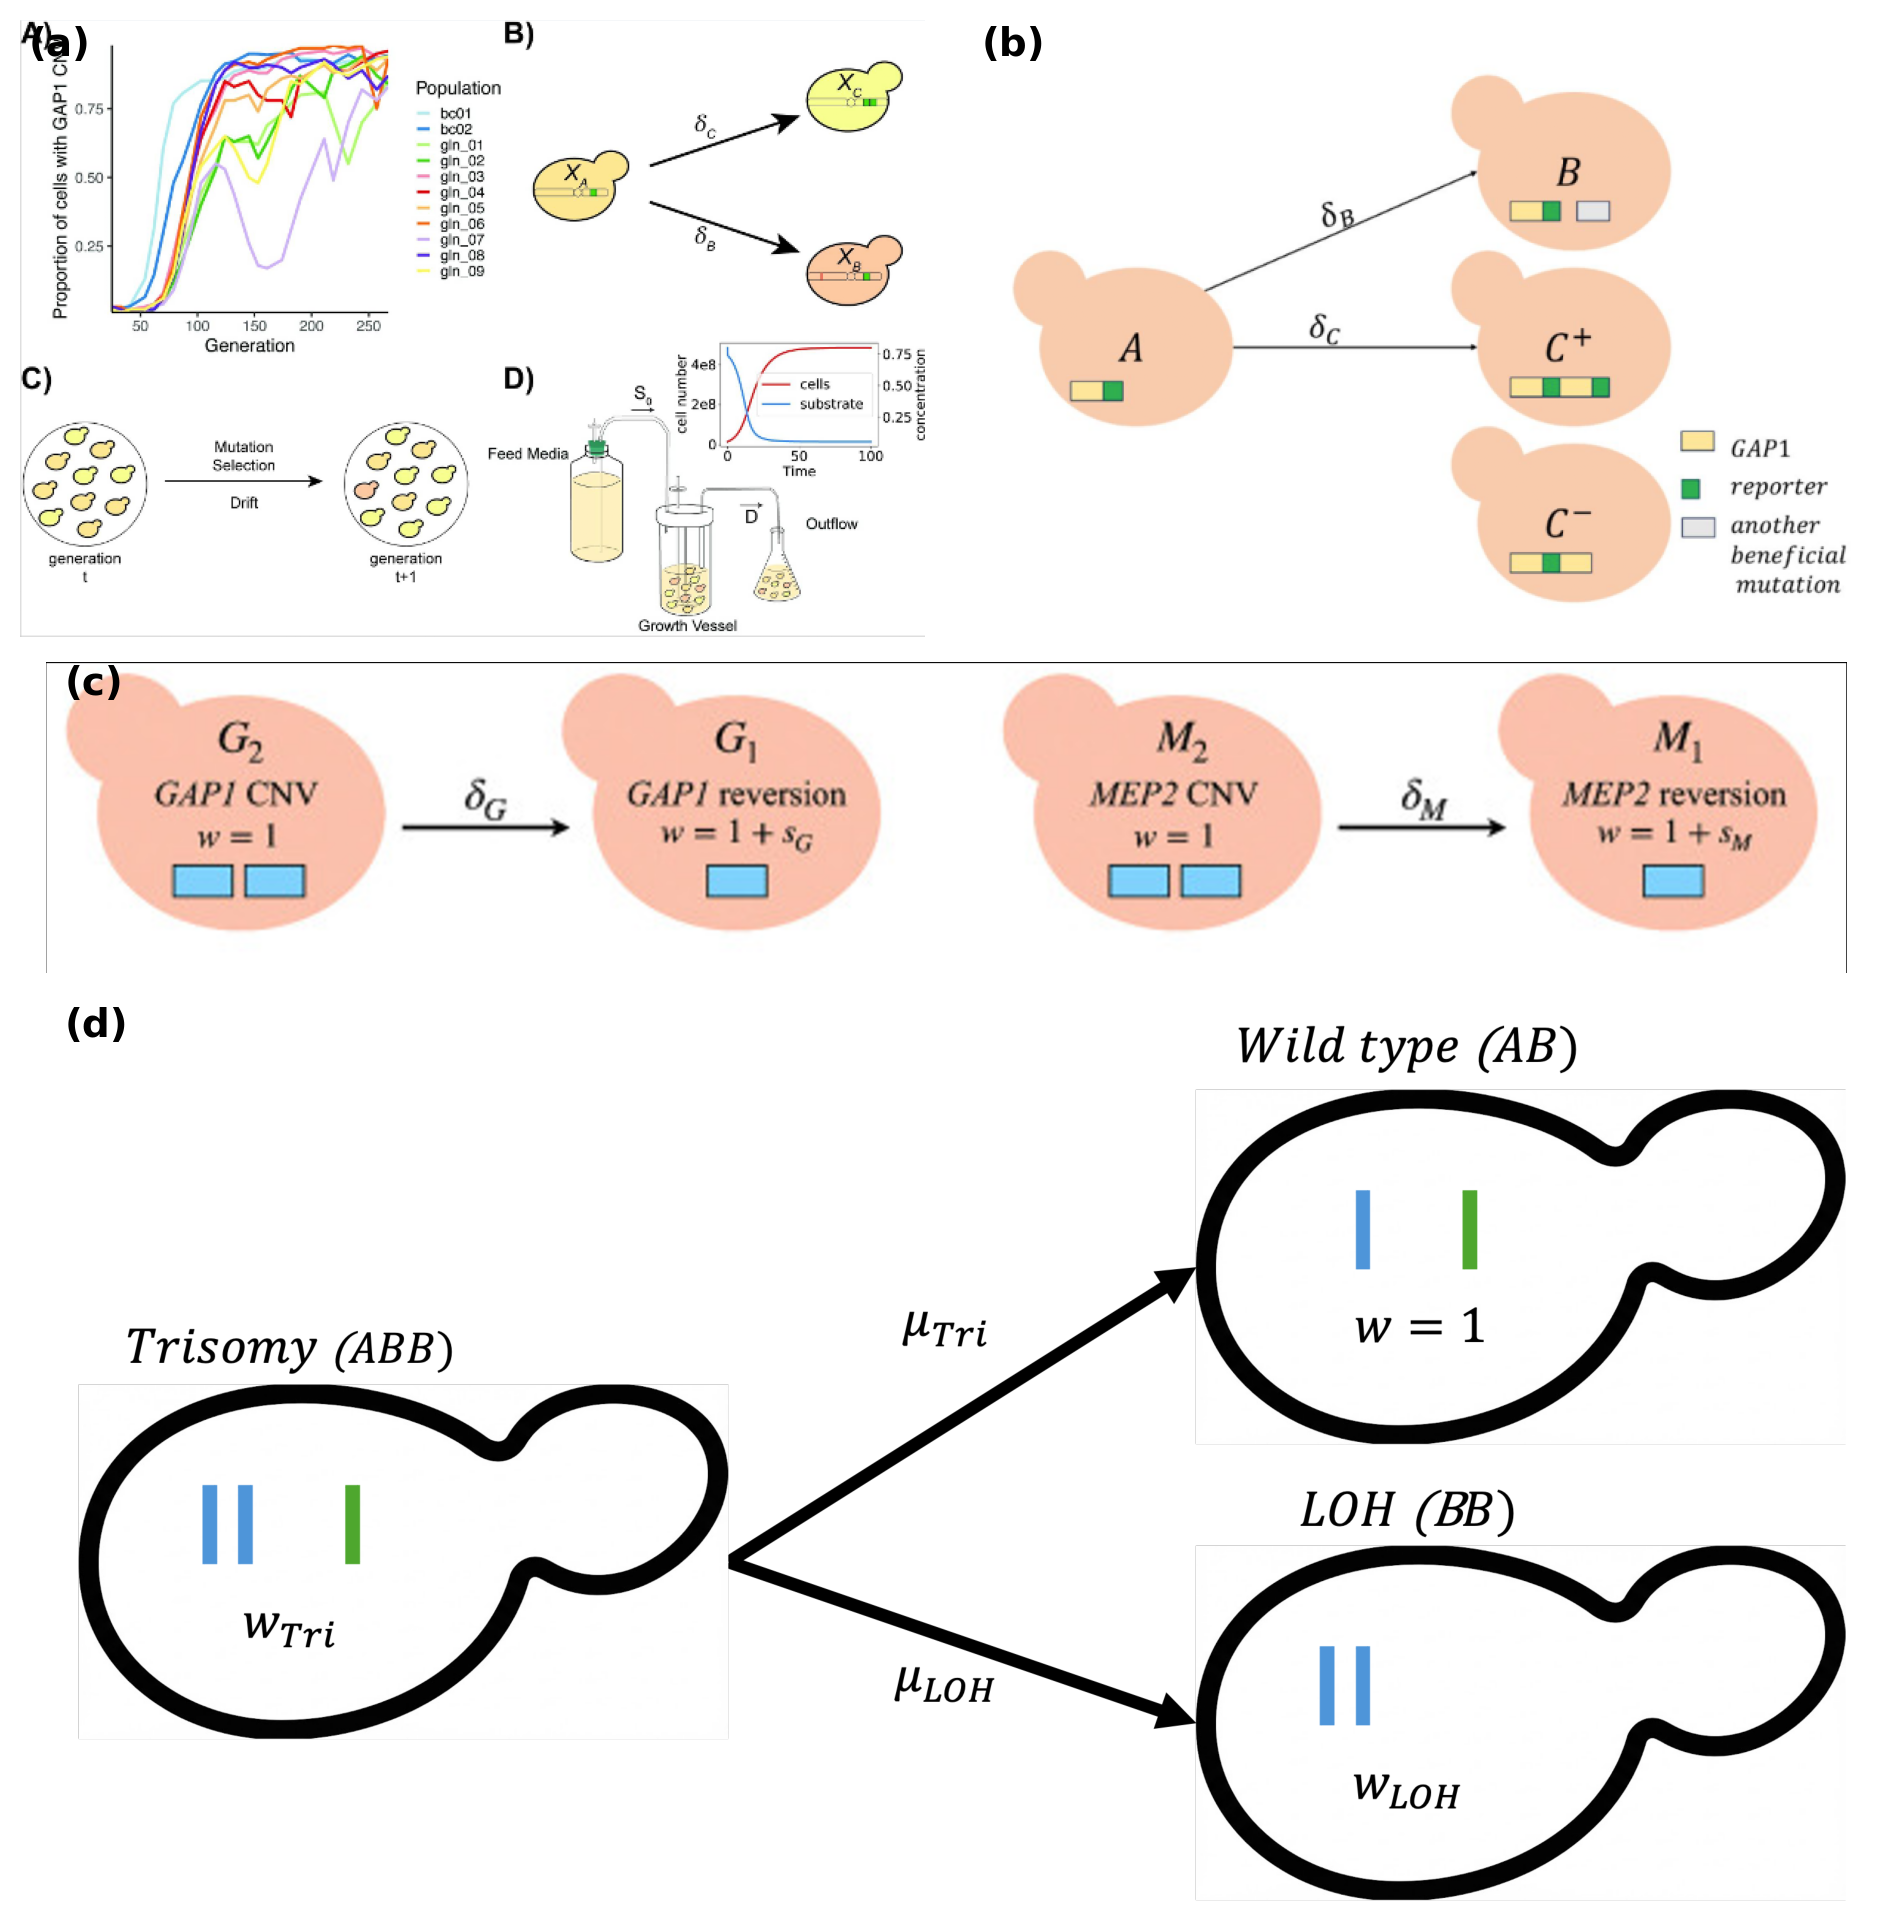
\includegraphics[width=\linewidth]{fig_model_schematics.png}
  \caption{\textbf{Wright-Fisher model schematics for four experimental
  systems.}
  (a)~Overview of the three-genotype chemostat model: empirical CNV
  frequency trajectories (top left), model schematic with ancestral
  ($X_A$), CNV ($X_C$), and other-beneficial-mutation ($X_B$) genotypes
  (top right), Wright-Fisher drift cartoon (bottom left), and chemostat
  bioreactor diagram (bottom right) \citep{avecilla2022neural}.
  (b)~Batch evolution model: WT, CNV\textsuperscript{$+$},
  CNV\textsuperscript{$-$}, and SNV genotypes; arrows show de-novo
  CNV formation (rate $\delta$) from the CNV\textsuperscript{$-$} pool
  \citep{chuong2025template}.
  (c)~Two-locus reversion model: GAP1 CNV ($G_2$) and MEP2 CNV ($M_2$)
  revert to single-copy genotypes ($G_1$, $M_1$) at rates $\delta_G$ and
  $\delta_M$ \citep{de2025segmental}.
  (d)~Aneuploidy stability model: trisomic cells (ABB) transition to
  diploid wild-type (AB) at rate $\mu_\mathrm{Tri}$ or to
  loss-of-heterozygosity (BB) at rate $\mu_\mathrm{LOH}$
  (Zhou et al., in prep.).
  Generated by \texttt{align\_figures.ipynb}.}
  \label{fig:model_schematics}
\end{figure}

\subsection{Aneuploidy stability model}
\label{sec:aneuploidy}

Whole-chromosome aneuploidy (gain or loss of a complete chromosome) is a
qualitatively different form of CNV.
Aneuploid cells are often unstable: a trisomic cell may revert to a diploid
or undergo loss of heterozygosity~(LOH) in a single step.
The three-genotype WF model for aneuploidy tracks the frequencies of trisomic
(Tri), diploid~(WT), and LOH cells, with transitions governed by rates
$\mu_\mathrm{tri}$ (Tri$\to$WT) and $\mu_\mathrm{loh}$ (Tri$\to$LOH), and
relative fitnesses $w_\mathrm{tri}$ and $w_\mathrm{loh}$
(Figure~\ref{fig:model_schematics}d).
All three genotype frequencies are observed simultaneously at six passages
(Zhou et al., in prep.).

\subsection{Chemostat ODE model}
\label{sec:ode}

An alternative to the discrete-generation WF model is a continuous-time ODE
that models the chemostat as a well-mixed bioreactor.
Nutrient-limited growth follows Monod kinetics,
$\mu_k = r_k S / (S + \kappa_k)$,
where $S$ is the substrate concentration, $r_k$ is the maximal growth rate,
and $\kappa_k$ is the half-saturation constant.
The ODE couples three genotype densities to the substrate balance equation.
Crucially, this model shares parameters with the WF chemostat model, allowing
cross-validation: Figure~\ref{fig:ode_vs_wf} shows that both models produce
nearly identical genotype-frequency trajectories when run with the same
inferred $\btheta$ \citep{avecilla2022neural}.
For practical inference we prefer the WF model because each trajectory
requires only milliseconds to simulate, while the ODE must be numerically
integrated at each parameter evaluation.

\begin{figure}[ht]
  \centering
  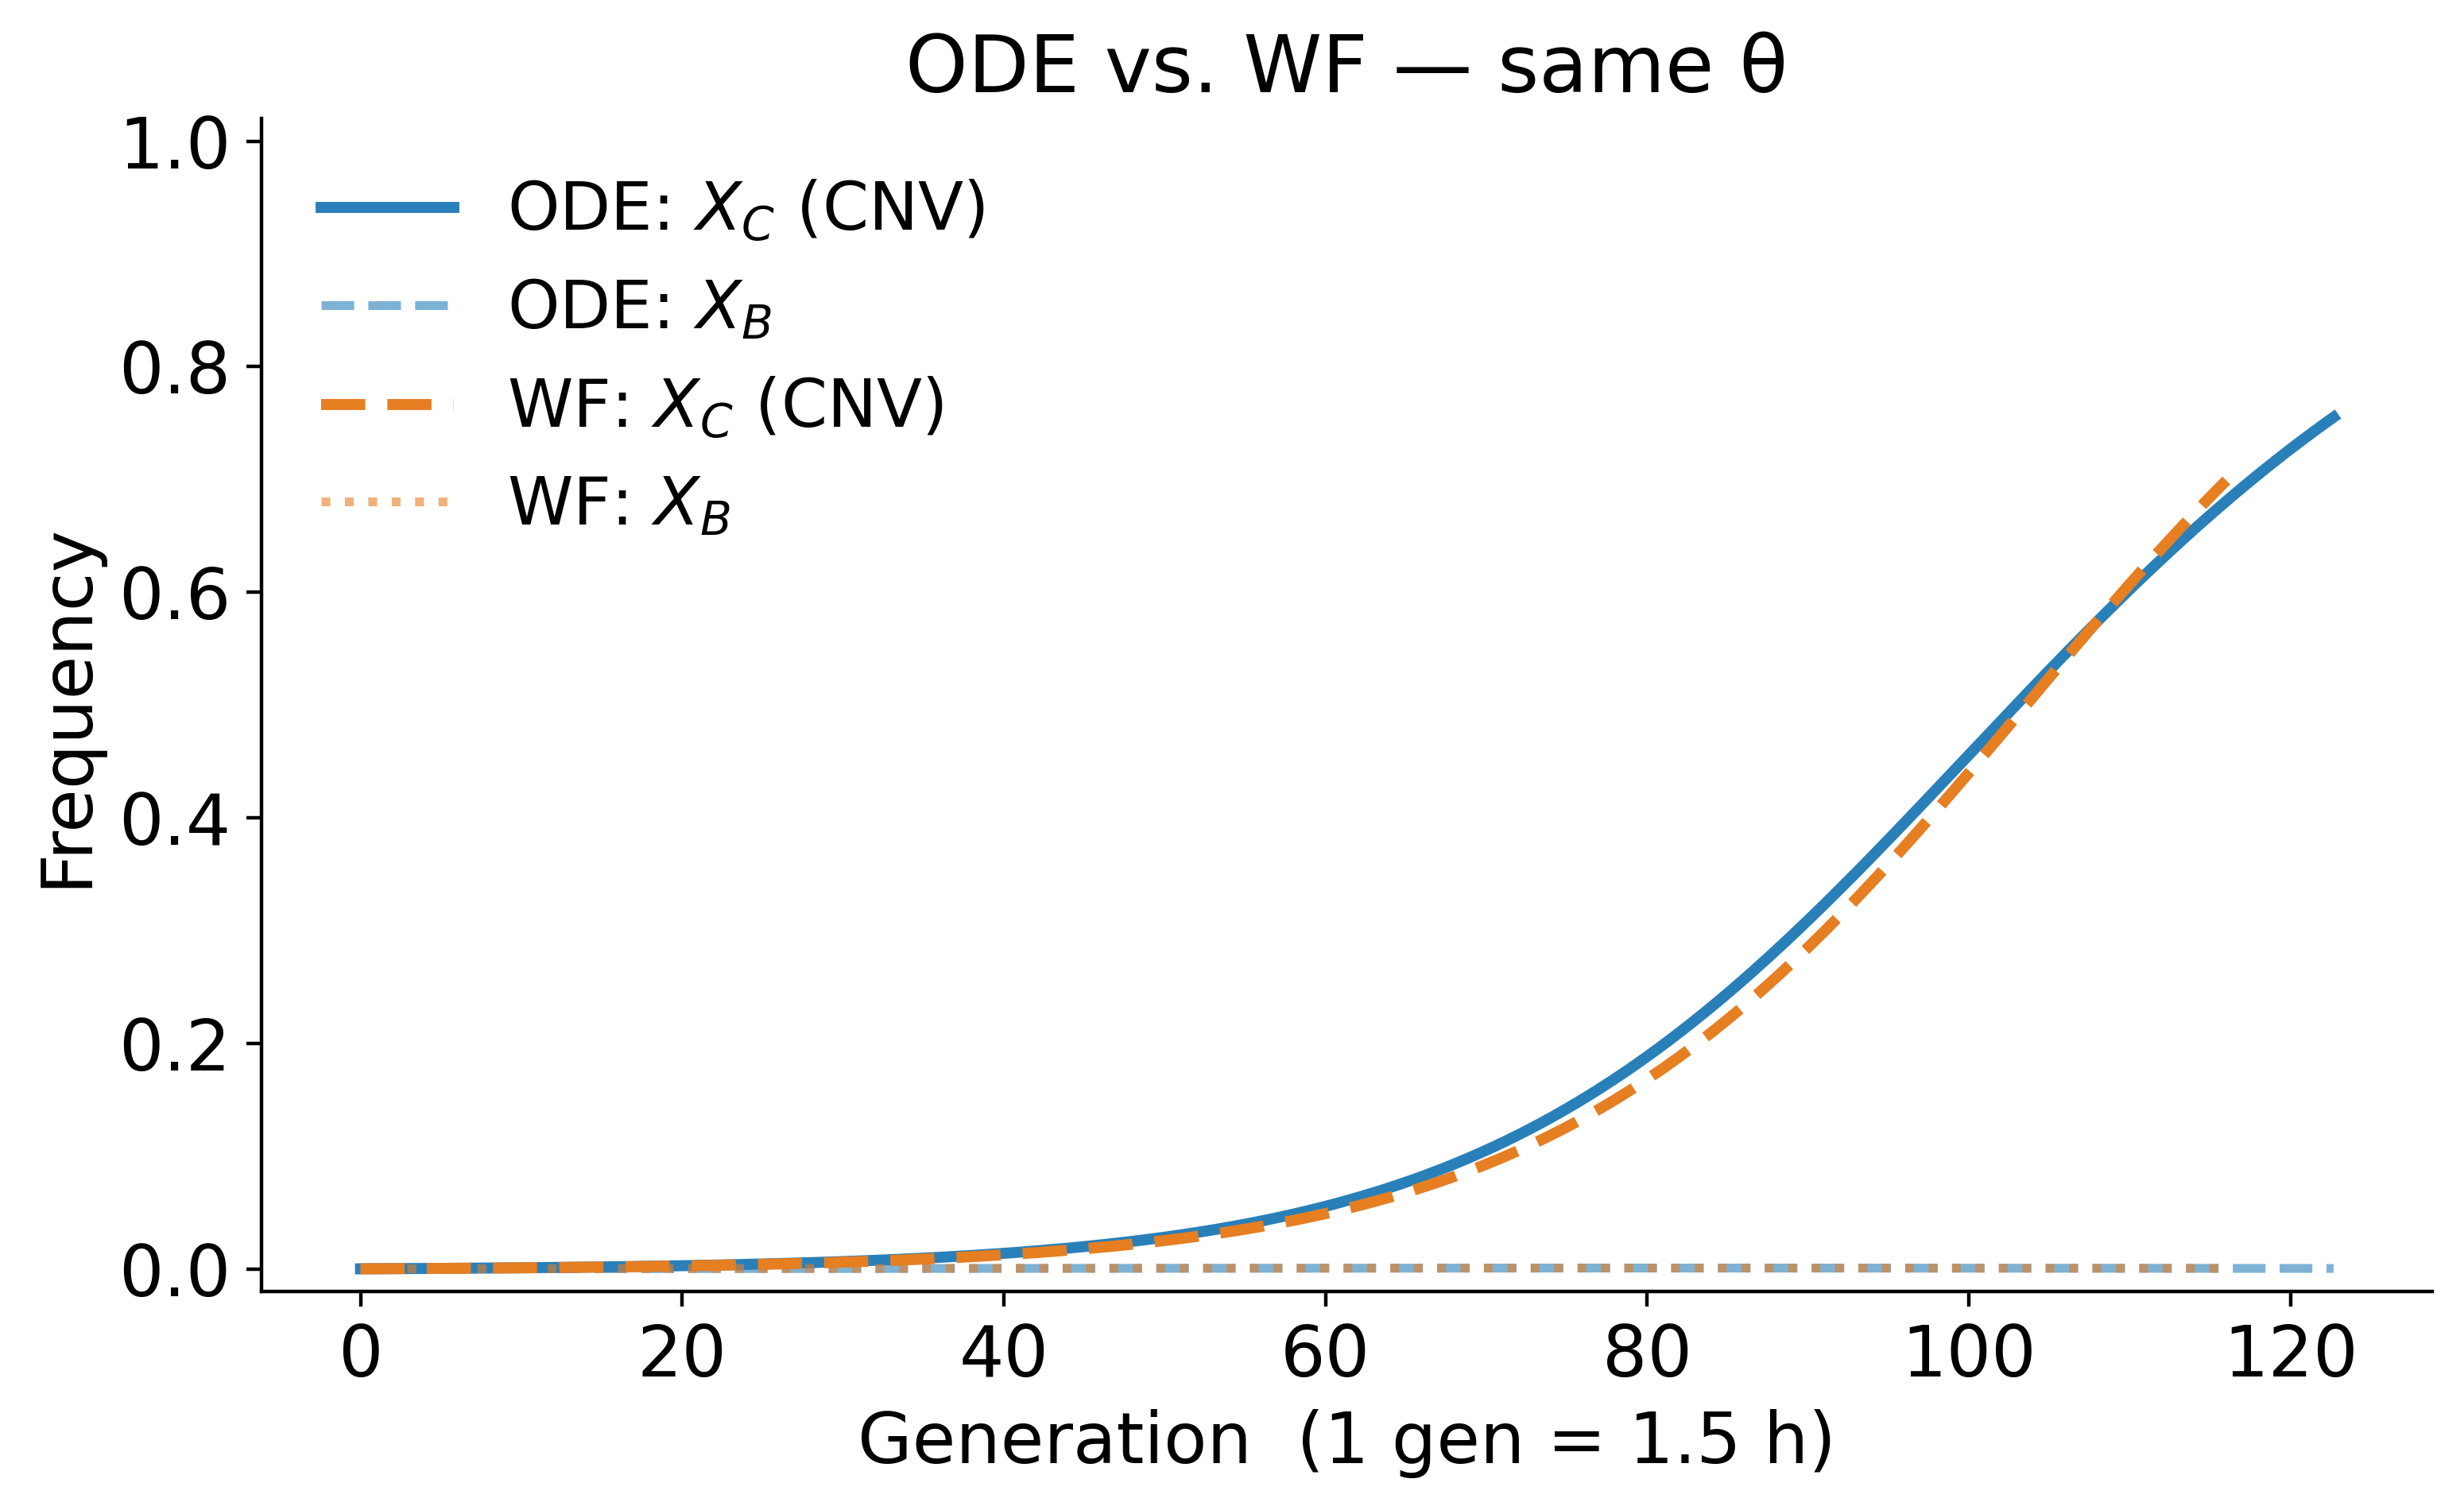
\includegraphics[width=0.6\linewidth]{fig_ode_vs_wf.png}
  \caption{\textbf{ODE and WF chemostat models produce equivalent trajectories
  at the same parameters.}
  CNV ($X_C$) and other-beneficial-mutation ($X_B$) frequencies simulated
  by the continuous-time ODE (solid lines) and the discrete-generation
  Wright-Fisher model (dashed/dotted lines) at the same parameter vector
  $\hat\btheta$.
  The two models are in close agreement throughout the trajectory, validating
  the WF model as a computationally efficient surrogate for the mechanistic
  ODE.
  (Generated by \texttt{evolution\_simulators.ipynb}.)}
  \label{fig:ode_vs_wf}
\end{figure}

% =============================================================================
\section{Simulation-Based Inference Methods}
\label{sec:sbi}
% =============================================================================

SBI encompasses a family of algorithms that share a common structure: a
forward simulator defines an implicit likelihood $p(\bx\mid\btheta)$, which
is never evaluated directly; instead, simulated pairs $(\btheta^{(i)},
\bx^{(i)})$ are used to approximate the posterior
$p(\btheta\mid\bx_\mathrm{obs})$.

\subsection{Approximate Bayesian Computation (ABC)}
\label{sec:abc}

ABC \citep{tavare1997inferring,pritchard1999population} is the oldest and most
conceptually transparent class of SBI algorithms.
The core idea is to approximate the intractable likelihood
$p(\bx\mid\btheta)$ by an acceptance criterion based on a distance
$\rho(\bx_\mathrm{sim}, \bx_\mathrm{obs})$ between simulated and observed data.

\begin{algorithm}[ht]
\caption{Rejection ABC}
\begin{algorithmic}[1]
  \Require Prior $p(\btheta)$, simulator $\mathcal{S}$, observed data
           $\bx_\mathrm{obs}$, number of simulations $N_\mathrm{sim}$,
           acceptance quantile $\alpha$
  \For{$i = 1$ to $N_\mathrm{sim}$}
    \State Sample $\btheta^{(i)} \sim p(\btheta)$
    \State Simulate $\bx^{(i)} \sim \mathcal{S}(\btheta^{(i)})$
    \State Compute $d^{(i)} = \rho(\bx^{(i)}, \bx_\mathrm{obs})$
  \EndFor
  \State Set threshold $\varepsilon = $ $\alpha$-quantile of $\{d^{(i)}\}$
  \State \Return $\{\btheta^{(i)} : d^{(i)} \le \varepsilon\}$ as
         approximate posterior samples
\end{algorithmic}
\label{alg:abc}
\end{algorithm}

In our setting the distance is the root-mean-squared error (RMSE) between
simulated and observed CNV frequency trajectories:
\begin{equation}
  \rho(\bx_\mathrm{sim}, \bx_\mathrm{obs})
  = \sqrt{\frac{1}{T}\sum_{t=1}^{T}(x_\mathrm{sim,t} - x_\mathrm{obs,t})^2}.
  \label{eq:rmse}
\end{equation}

The acceptance quantile $\alpha$ controls the precision--recall trade-off.
With $N_\mathrm{sim} = 30{,}000$ and $\alpha = 0.02$, the accepted set
contains 600 approximate posterior samples.
ABC makes no parametric assumptions about the posterior shape, and the
algorithm is trivially parallelisable.
Its principal limitation is \emph{sample inefficiency}: nearly all computation
is discarded, and the approximation quality degrades as the data dimension $T$
grows, because the probability that $\rho < \varepsilon$ shrinks exponentially
fast in $T$ (the curse of dimensionality for ABC).
Summary statistics that compress $\bx$ to a lower-dimensional representation
can mitigate this, but choosing good summaries is problem-specific
\citep{beaumont2002approximate}.

\subsection{Sequential ABC methods}
\label{sec:seq_abc}

The efficiency of rejection ABC can be improved by adapting the proposal
distribution to concentrate mass near the posterior.
ABC-MCMC \citep{marjoram2003markov} embeds ABC within a Metropolis-Hastings
chain, so that proposals are accepted or rejected based on
$\rho < \varepsilon$ instead of an exact likelihood ratio.
Sequential Monte Carlo ABC (ABC-SMC) \citep{sisson2007sequential,
del2012adaptive} anneals a sequence of decreasing thresholds
$\varepsilon_1 > \varepsilon_2 > \cdots > \varepsilon_G$, using a
population of particles that is sequentially refined through importance
reweighting and MCMC rejuvenation.
ABC-SMC typically requires an order of magnitude fewer simulations than
rejection ABC to achieve the same posterior approximation quality, but
introduces tuning parameters (number of particles, perturbation kernel,
schedule of $\varepsilon$ values) and is more complex to implement.

\subsection{Neural Posterior Estimation (NPE)}
\label{sec:npe}

Neural Posterior Estimation (NPE) replaces the non-parametric accept/reject
criterion of ABC with a \emph{learned} conditional density estimator
$q_\phi(\btheta\mid\bx)$ \citep{papamakarios2016fast,lueckmann2017flexible,
greenberg2019automatic}.
This estimator is trained by maximising the expected log-posterior:
\begin{equation}
  \mathcal{L}(\phi) = \E_{p(\btheta)p(\bx\mid\btheta)}
    \bigl[\log q_\phi(\btheta\mid\bx)\bigr].
  \label{eq:npe_loss}
\end{equation}

In practice, $q_\phi$ is implemented as a \emph{normalizing flow}
\citep{papamakarios2021normalizing}---a neural network that maps a simple base
distribution (e.g., a standard Gaussian) to a complex, data-conditioned
density via a sequence of invertible transformations.
We use a Masked Autoregressive Flow (MAF), which expresses the joint density
of $\btheta = (\theta_1,\ldots,\theta_d)$ as a product of conditionals,
each modelled by a single-hidden-layer autoregressive network.

\paragraph{Amortisation.}
A decisive advantage of NPE over ABC is \emph{amortised inference}: once the
network is trained on $N_\mathrm{sim}$ simulations, evaluating
$q_\phi(\btheta\mid\bx_\mathrm{obs})$ for a new observation $\bx_\mathrm{obs}$
requires only a single forward pass (milliseconds), regardless of how
many new datasets are to be analysed.
This is ideal for experimental evolution, where the same simulator is applied
to many replicate trajectories from the same experimental system.

\paragraph{Observation noise.}
Flow cytometry measurements contain technical noise on top of evolutionary
stochasticity.
We model this by adding Gaussian noise $\varepsilon_t\sim\mathcal{N}(0,
\sigma^2)$ to each simulated frequency, with $\sigma = 0.02$ calibrated to
the empirical measurement noise in our datasets.
This ensures that the learned posterior accounts for both biological and
technical variability.

\paragraph{Sequential variants.}
The original NPE (SNPE-A) proposes from the prior at every round and corrects
for the resulting importance-sampling mismatch via an approximate ratio
\citep{papamakarios2016fast}.
SNPE-B refines proposals using a mixture density network and applies an
explicit proposal correction \citep{lueckmann2017flexible}.
SNPE-C (APT) eliminates the need for explicit corrections by using an atomic
proposal and optimising a lower bound on the marginal log-likelihood
\citep{greenberg2019automatic}, and is the current default in the \texttt{sbi}
package \citep{tejero2020sbi}.
Sequential methods use the approximated posterior from round $r$ as the
proposal for round $r+1$, concentrating simulations near the true posterior.
In the low-budget regime this can yield substantial gains; for our
experiments, a single round with $N_\mathrm{sim}=30{,}000$ suffices because
the prior is already reasonably informative.

\subsection{Neural Likelihood Estimation (NLE)}
\label{sec:nle}

Instead of directly estimating the posterior, Neural Likelihood Estimation
(NLE) learns the simulator's likelihood $p(\bx\mid\btheta)$
\citep{papamakarios2019sequential}.
A normalizing flow $q_\phi(\bx\mid\btheta)$ is trained by maximising
$\E[\log q_\phi(\bx\mid\btheta)]$ over simulated pairs.
Once trained, $q_\phi(\bx_\mathrm{obs}\mid\btheta)$ serves as a
plug-in likelihood in any MCMC sampler.
NLE is especially useful when one wishes to incorporate structured priors
or physical constraints that are difficult to encode into a normalizing-flow
posterior, since the prior enters naturally into the MCMC acceptance step.
Its main disadvantage is that posterior evaluation still requires MCMC, which
is slower than NPE's single forward pass.
Sequential NLE (SNLE) refines proposals across rounds analogously to SNPE.

\subsection{Neural Likelihood-Ratio Estimation (NRE)}
\label{sec:nre}

Neural Ratio Estimation (NRE) \citep{hermans2020likelihood} frames inference
as a binary classification problem: given a pair $(\btheta, \bx)$, does it
come from the joint $p(\btheta)p(\bx\mid\btheta)$ or from the product of
marginals $p(\btheta)p(\bx)$?
A classifier trained to distinguish these two classes learns the
\emph{likelihood-to-evidence ratio}
$r(\btheta, \bx) = p(\bx\mid\btheta)/p(\bx)$,
from which the posterior follows as
$p(\btheta\mid\bx) \propto p(\btheta)\,r(\btheta,\bx)$.
NRE is particularly attractive when the parameter-to-data mapping is
high-dimensional or the likelihood surface is multimodal, because classifiers
can be expressive without requiring the density to be normalised.
Sequential versions (SNRE) progressively sharpen the ratio estimate.

\subsection{Practical comparison}
\label{sec:comparison}

Table~\ref{tab:sbi_comparison} summarises the key trade-offs among the
methods discussed above.
For experimental evolution with moderate data dimensionality
($T \lesssim 20$ time points, $d \lesssim 4$ parameters), we recommend NPE
as the default choice for the following reasons:
\begin{itemize}
  \item Posterior evaluation is amortised, making per-replicate inference
        essentially free once training is complete.
  \item MAF-based normalizing flows handle log-scaled parameters and
        multi-modal posteriors gracefully.
  \item The \texttt{sbi} package \citep{tejero2020sbi} provides a
        straightforward implementation with sensible defaults.
\end{itemize}
ABC remains the simplest entry point and should be used for quick
prototyping or when the simulation budget is small (hundreds to a few
thousand simulations), as training a neural network on fewer simulations
tends to overfit.
NLE is preferred when the prior is non-standard or when one wants to
augment the learned likelihood with physically motivated constraints.
NRE is particularly well suited to high-dimensional data or when the
likelihood-to-evidence ratio is easier to learn than the full likelihood
or posterior.

Figure~\ref{fig:abc_vs_npe} illustrates the NPE--ABC comparison on a
synthetic dataset drawn from the four-genotype batch model.

\begin{table}[ht]
  \centering
  \caption{\textbf{Comparison of SBI methods.}
  ``Amortised'' means posterior evaluation for new observations requires
  no additional simulations after training.
  ``Sequential'' means multiple rounds of simulation with adaptive proposals.}
  \label{tab:sbi_comparison}
  \begin{tabular}{lccccl}
    \toprule
    Method & Amortised & Sequential & Trains on & MCMC needed & Notes \\
    \midrule
    Rejection ABC        & No  & No       & Raw data  & No  & Simplest baseline \\
    ABC-SMC              & No  & Yes      & Raw data  & No  & Better efficiency \\
    ABC-MCMC             & No  & No       & Raw data  & Yes & Slow mixing \\
    NPE (SNPE-A/B/C)     & Yes & Optional & Raw data  & No  & \textbf{Recommended} \\
    NLE / SNLE           & No  & Optional & Raw data  & Yes & Flexible prior \\
    NRE / SNRE           & No  & Optional & Pairs     & Yes & High-dim data \\
    \bottomrule
  \end{tabular}
\end{table}

\begin{figure}[ht]
  \centering
  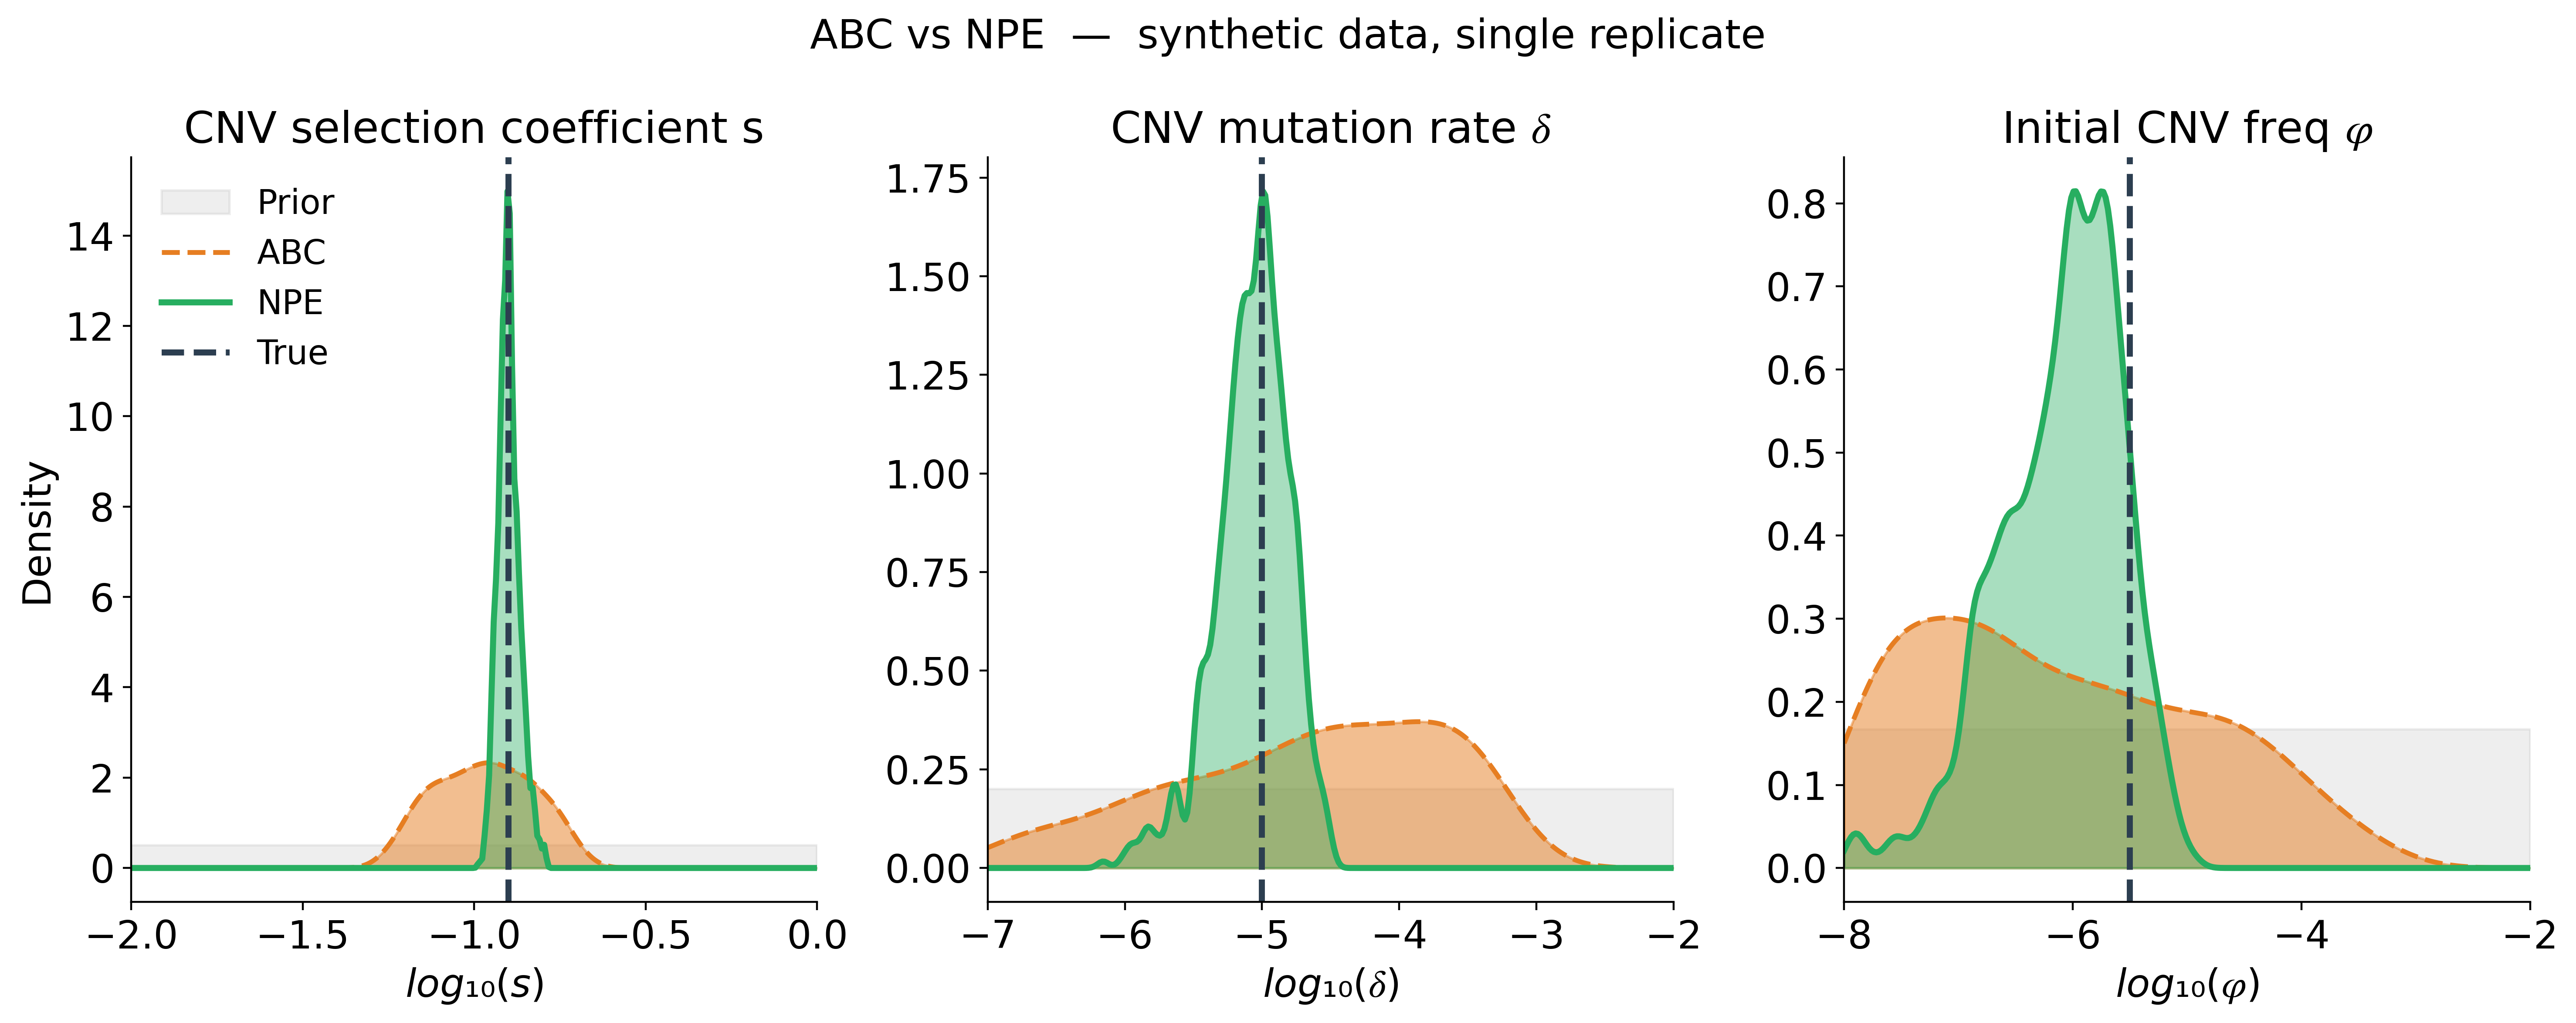
\includegraphics[width=\linewidth]{fig_abc_vs_npe.png}
  \caption{\textbf{Posterior comparison: rejection ABC vs.\ NPE on synthetic
  data.}
  Marginal posterior densities for the three inferred parameters
  ($\log_{10} s$, $\log_{10}\delta$, $\log_{10}\varphi$) for a single
  synthetic observation drawn from the four-genotype batch model
  \citep{chuong2025template}.
  Both methods use $N_\mathrm{sim}=30{,}000$ simulations from the prior.
  The grey shading shows the prior; orange shows the ABC posterior; green
  shows the NPE posterior; the dashed vertical line marks the true parameter
  value.
  NPE produces a substantially tighter and better-calibrated posterior than
  rejection ABC with the same simulation budget.
  (Generated by \texttt{SBI\_tutorial.ipynb}.)}
  \label{fig:abc_vs_npe}
\end{figure}

% =============================================================================
\section{Multi-Replicate Inference: Summary of Companion Work}
\label{sec:collective}
% =============================================================================

The material in this section provides context for one important extension of
the single-replicate SBI workflow developed in this paper.
Because multi-replicate aggregation is a substantial topic in its own right,
we treat it here as companion methodology rather than as the main research
contribution of the present manuscript.

\subsection{The multi-replicate problem}
\label{sec:multi_rep_problem}

Experimental evolution studies routinely generate $r = 4$--$20$ replicate
populations evolved under identical conditions.
Each replicate trajectory $\bx_i$ contains independent information about the
same underlying parameter vector~$\btheta$.
Naively, one could infer parameters from each replicate independently and
then average the resulting posteriors.
This is incorrect, however, because an average of posteriors is not a
posterior---it over-counts the prior.
The correct approach is to \emph{multiply} the likelihoods across replicates,
which yields a much sharper combined posterior.

\subsection{Derivation of the collective posterior}
\label{sec:collective_derivation}

Assume the $r$ replicate trajectories are conditionally independent given
$\btheta$:
\begin{equation}
  p(\bx_1,\ldots,\bx_r\mid\btheta) = \prod_{i=1}^{r} p(\bx_i\mid\btheta).
  \label{eq:likelihood_product}
\end{equation}
By Bayes' theorem the joint posterior is
\begin{equation}
  p(\btheta\mid\bx_1,\ldots,\bx_r)
  \propto p(\btheta)\prod_{i=1}^{r} p(\bx_i\mid\btheta).
  \label{eq:joint_posterior}
\end{equation}
NPE gives us an amortised approximation $q_\phi(\btheta\mid\bx_i)$ to each
individual posterior
$p_i(\btheta\mid\bx_i) \propto p(\btheta)\,p(\bx_i\mid\btheta)$.
We can write
\begin{equation}
  p(\bx_i\mid\btheta) \;\propto\;
  \frac{p_i(\btheta\mid\bx_i)}{p(\btheta)},
  \label{eq:likelihood_from_posterior}
\end{equation}
and substituting into (\ref{eq:joint_posterior}):
\begin{equation}
  p(\btheta\mid\bx_1,\ldots,\bx_r)
  \;\propto\; p(\btheta)^{1-r}\,\prod_{i=1}^{r} p_i(\btheta\mid\bx_i).
  \label{eq:collective_unnorm}
\end{equation}
Taking logarithms and replacing each $p_i$ by its learned approximation
$q_\phi(\cdot\mid\bx_i)$:
\begin{equation}
  \boxed{
  \log p(\btheta\mid\bx_1,\ldots,\bx_r)
  = \sum_{i=1}^{r} \log q_\phi(\btheta\mid\bx_i)
    - (r-1)\log p(\btheta) - \log C,
  }
  \label{eq:collective_log}
\end{equation}
where $C$ is a normalising constant estimated by importance sampling from the
prior.
Equation~(\ref{eq:collective_log}) is the \emph{collective posterior}
\citep{bennun2026collective}.

\paragraph{Why not average posteriors?}
An average of individual posteriors weights each replicate's evidence equally
but retains $r$ copies of the prior, effectively over-regularising toward
$p(\btheta)$ as the number of replicates grows.
Equation~(\ref{eq:collective_log}) correctly cancels $r-1$ copies of the
prior, so the collective posterior narrows at the statistically optimal rate
$\sigma \propto r^{-1/2}$ as the number of replicates increases.
Figure~\ref{fig:collective_synthetic} demonstrates this on eight synthetic
replicates.

\begin{figure}[ht]
  \centering
  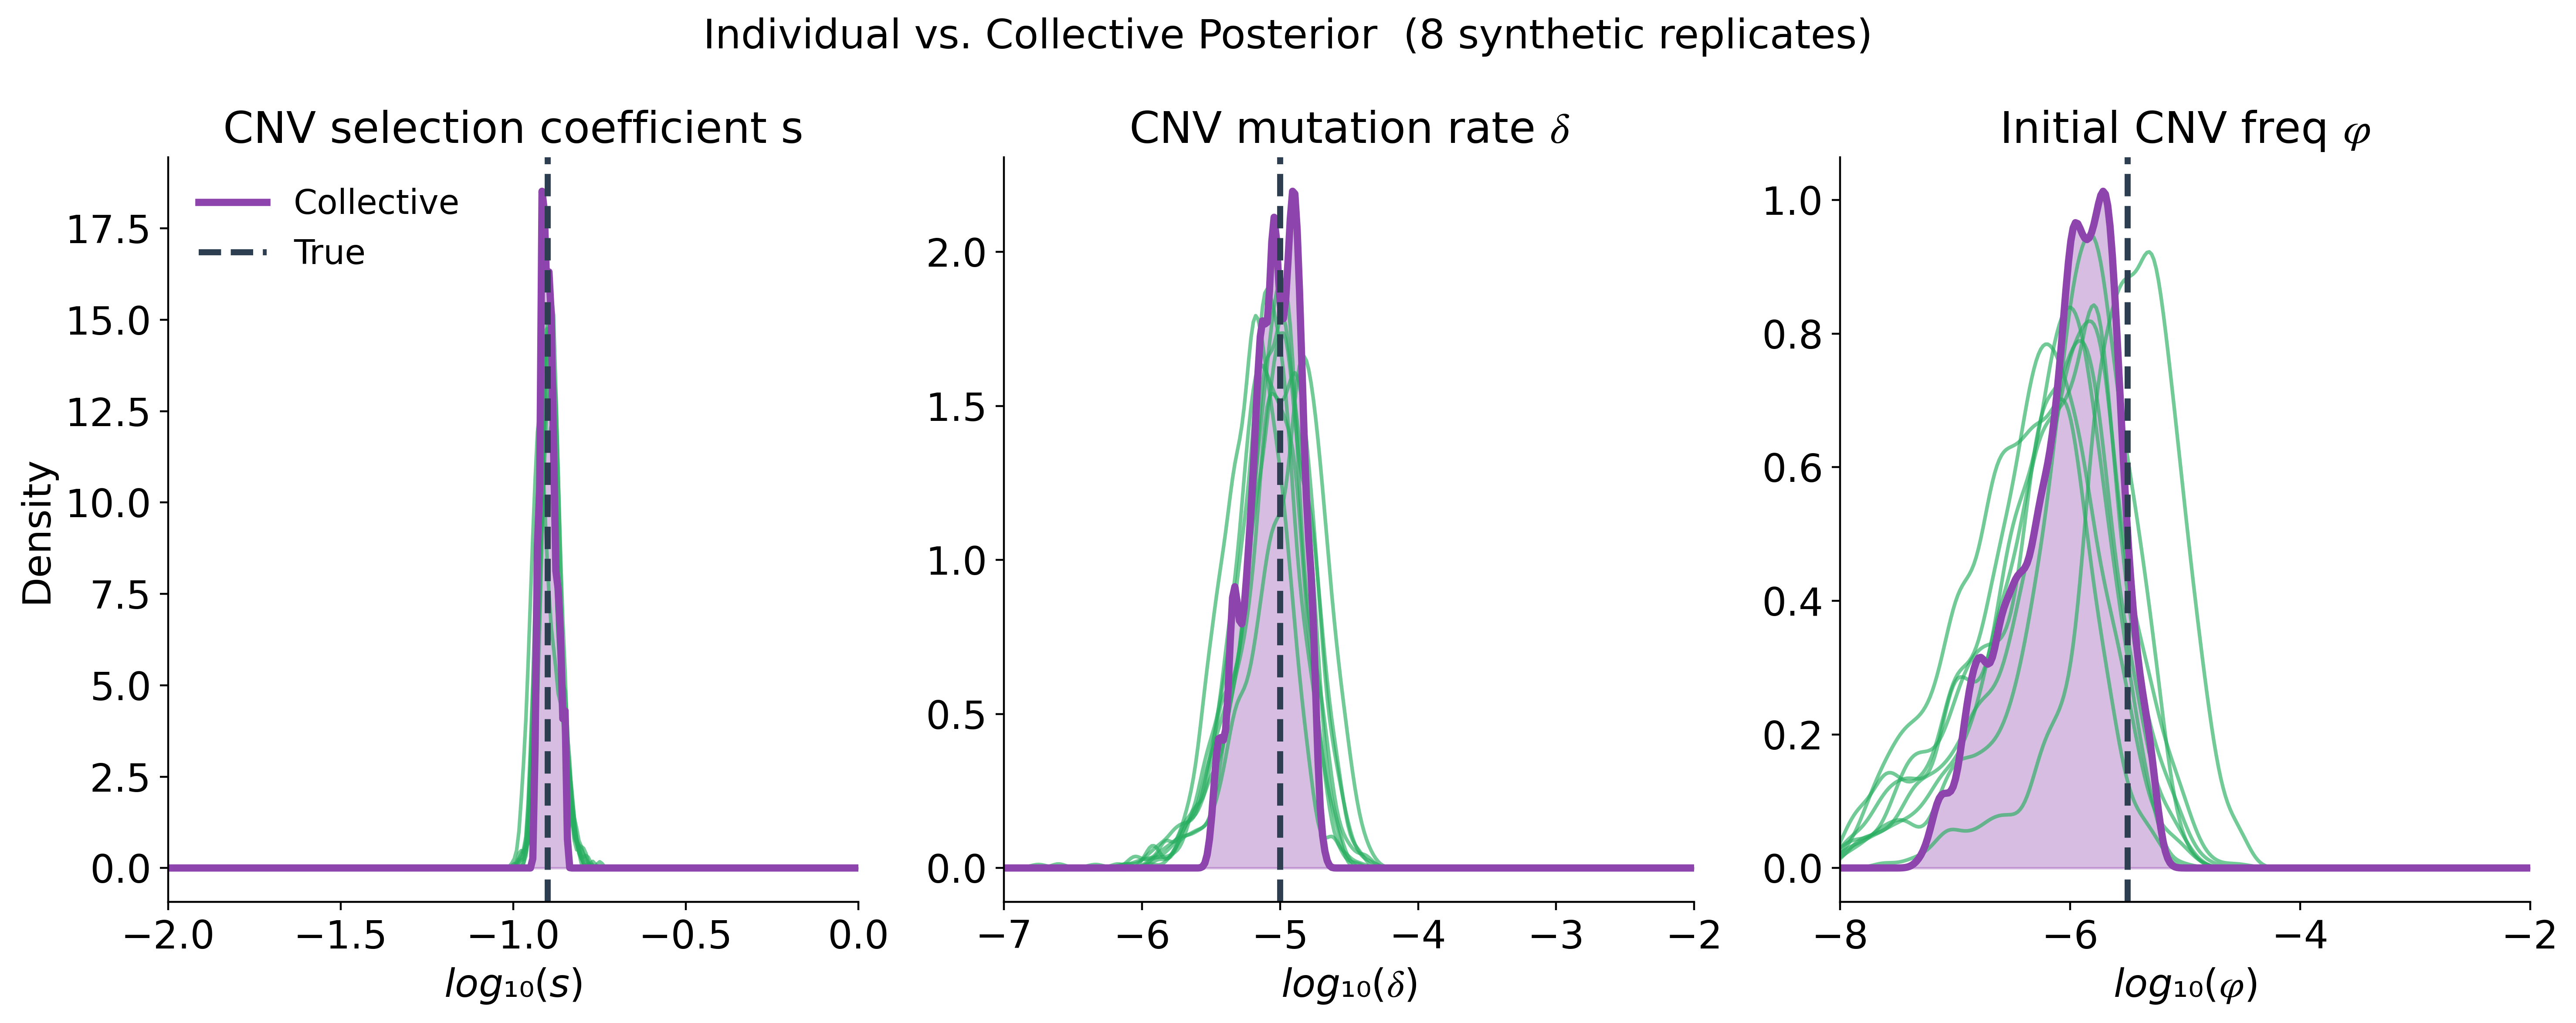
\includegraphics[width=\linewidth]{fig_collective_synthetic.png}
  \caption{\textbf{Individual and collective posteriors for eight synthetic
  replicates.}
  Marginal posterior densities for $\log_{10} s$, $\log_{10}\delta$, and
  $\log_{10}\varphi$ across eight independently simulated replicates from the
  four-genotype batch model at a fixed ``true'' $\btheta$ (dashed vertical
  line).
  Individual NPE posteriors (green) vary due to genetic drift between
  replicates; the collective posterior (purple) is substantially narrower
  than any single replicate's posterior, consistent with the expected
  $r^{-1/2}$ narrowing for $r=8$ replicates.
  (Generated by \texttt{SBI\_tutorial.ipynb}.)}
  \label{fig:collective_synthetic}
\end{figure}

\subsection{Robust collective inference}
\label{sec:robust_collective}

In practice some replicates may be outliers: their trajectories may be
dominated by a single large-effect mutation that does not represent the
target system, by a measurement artefact, or by an atypical founder effect.
Outlier replicates pull the joint likelihood product away from the consensus,
inflating uncertainty or biasing estimates.
\citet{bennun2026collective} address this with a \emph{robust product-of-experts}
scheme that replaces the sum in (\ref{eq:collective_log}) with a
trimmed or soft-thresholded aggregation, automatically down-weighting
replicates whose individual log-posterior differs substantially from the
consensus.
We implement the simple version of (\ref{eq:collective_log}) in the tutorial
notebook; readers requiring robustness should consult \citet{bennun2026collective}
for the full implementation.

\subsection{Sampling the collective posterior}
\label{sec:collective_sampling}

The collective posterior (\ref{eq:collective_log}) is not represented in
closed form; we draw samples from it using either:
\begin{enumerate}
  \item \textbf{Rejection sampling.} Draw $\btheta' \sim p(\btheta)$, accept
        with probability proportional to the unnormalised density.
        Efficient when $\log C$ is not too negative (i.e., the prior and
        collective posterior overlap well).
  \item \textbf{MCMC.} Metropolis-Hastings chains initialised from the
        top-probability prior samples found during the importance-sampling
        estimation of $C$.
        Preferred when the collective posterior is much narrower than the
        prior.
\end{enumerate}

% =============================================================================
\section{Results Across Experimental Systems}
\label{sec:applications}
% =============================================================================

We now evaluate the SBI workflow across four experimental systems.
The goal of this section is not only to demonstrate that inference can be
performed, but to identify what the examples reveal about reliability.
Across these systems we use posterior shape, posterior-predictive fit, and
cross-model comparison to study three recurring issues:
how strongly the posterior depends on the prior, how stable inference is
across estimators, and how visible model misspecification becomes once one
checks simulated trajectories against data.
Figure~\ref{fig:four_simulators} provides an overview of the simulator family
and their empirical fits.

\begin{figure}[ht]
  \centering
  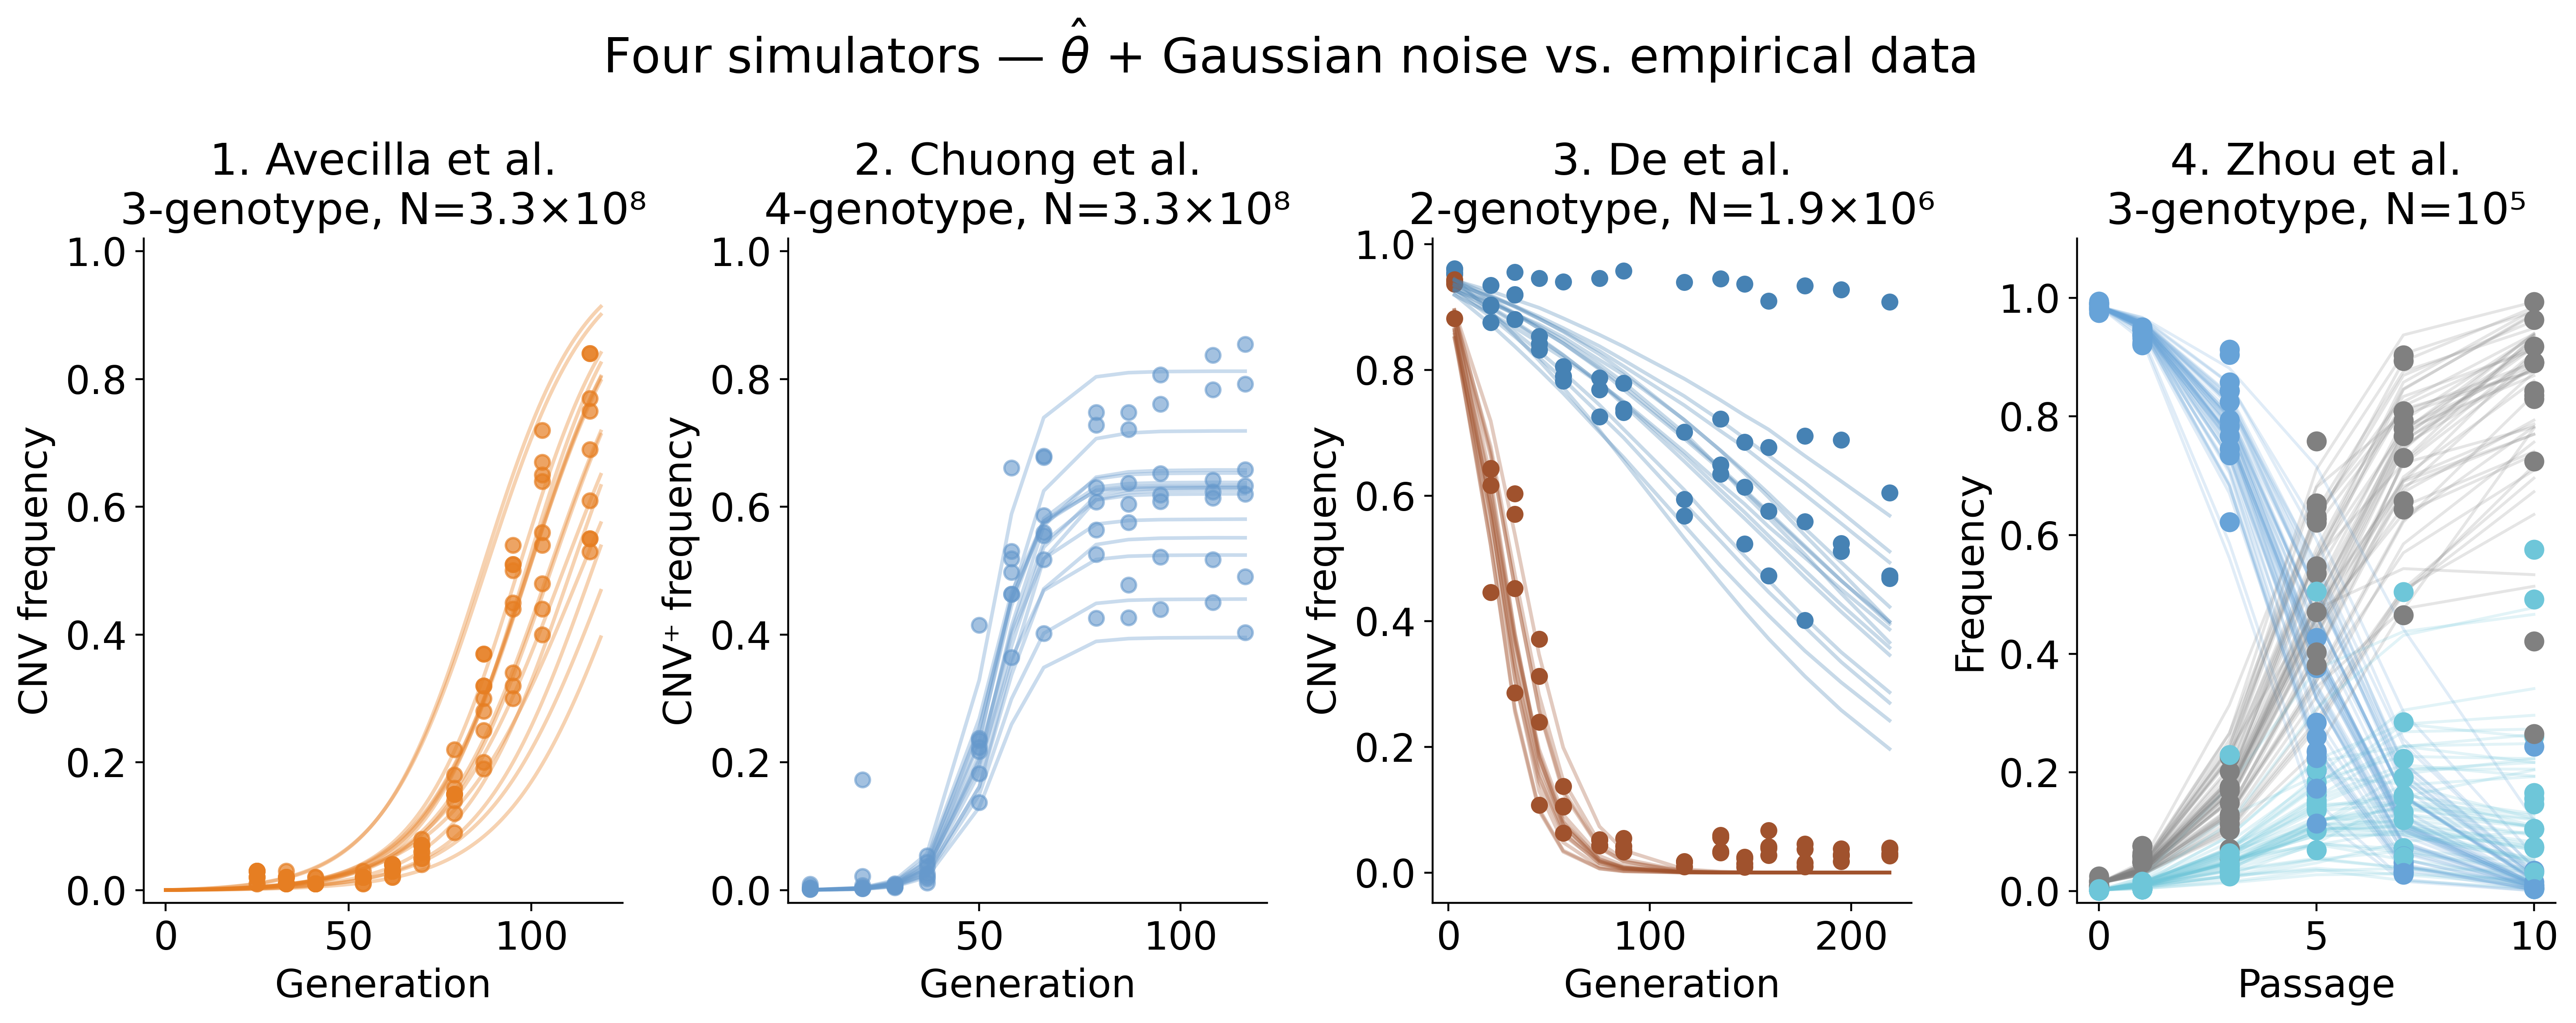
\includegraphics[width=\linewidth]{fig_four_simulators.png}
  \caption{\textbf{Overview of all four evolutionary simulators applied to
  empirical data.}
  Each panel shows CNV or genotype-frequency trajectories from a distinct
  experimental system (dots = data, lines = simulations from
  $\hat\btheta + \text{Gaussian noise}$).
  Panel~1: three-genotype chemostat model fit to nine \emph{S. cerevisiae}
  replicate populations from \citet{avecilla2022neural}.
  Panel~2: four-genotype batch model fit to LTRΔ replicates from
  \citet{chuong2025template}.
  Panel~3: two-genotype reversion model fit to \emph{GAP1} and \emph{MEP2}
  CNV lineages from \citet{de2025segmental}.
  Panel~4: three-genotype aneuploidy model fit to Chr5 trisomic lineages
  (Zhou et al., in prep.).
  Effective population sizes $N$ are indicated above each panel.
  (Generated by \texttt{evolution\_simulators.ipynb}.)}
  \label{fig:four_simulators}
\end{figure}

\subsection{CNV adaptation in nutrient-limited chemostats (Avecilla et al.\ 2022)}
\label{sec:avecilla}

\subsubsection{System and data}

\citet{avecilla2022neural} studied \emph{S. cerevisiae} populations evolving
in glutamine-limited chemostats.
A fluorescent CNV reporter tracked the frequency of \emph{GAP1}
copy-number amplifications across nine replicate populations at 11 time
points.
This dataset was the first to be analysed with NPE in an evolutionary
context.

\subsubsection{Simulator and prior}

We use the three-genotype WF chemostat model
(Section~\ref{sec:cnv_models}, Figure~\ref{fig:model_schematics}a) with
$N = 3.3\times10^8$.
The prior is log-uniform for mutation rates and uniform for selection
coefficients:
$\log\delta_C \sim \mathcal{U}(-8, -3)$,
$\log\delta_B \sim \mathcal{U}(-8, -3)$,
$s_C \sim \mathcal{U}(0, 0.2)$,
$s_B \sim \mathcal{U}(0, 0.4)$.

\subsubsection{Model fit and results}

Figure~\ref{fig:avecilla_wf_fit} shows the chemostat model fit to all nine
replicate trajectories from \citet{avecilla2022neural}, together with a
single forward simulation of all three genotypes.
The inferred CNV formation rate at the \emph{GAP1} locus is
$\hat\delta_C \approx 10^{-4.7}$--$10^{-4}$ per cell division, and the
fitness coefficient is $\hat s_C \approx 0.04$--$0.1$ per generation.
These estimates were independently validated by barcode lineage tracking and
pairwise fitness assays, confirming that NPE with the WF chemostat model
produces accurate, well-calibrated posteriors \citep{avecilla2022neural}.

\begin{figure}[ht]
  \centering
  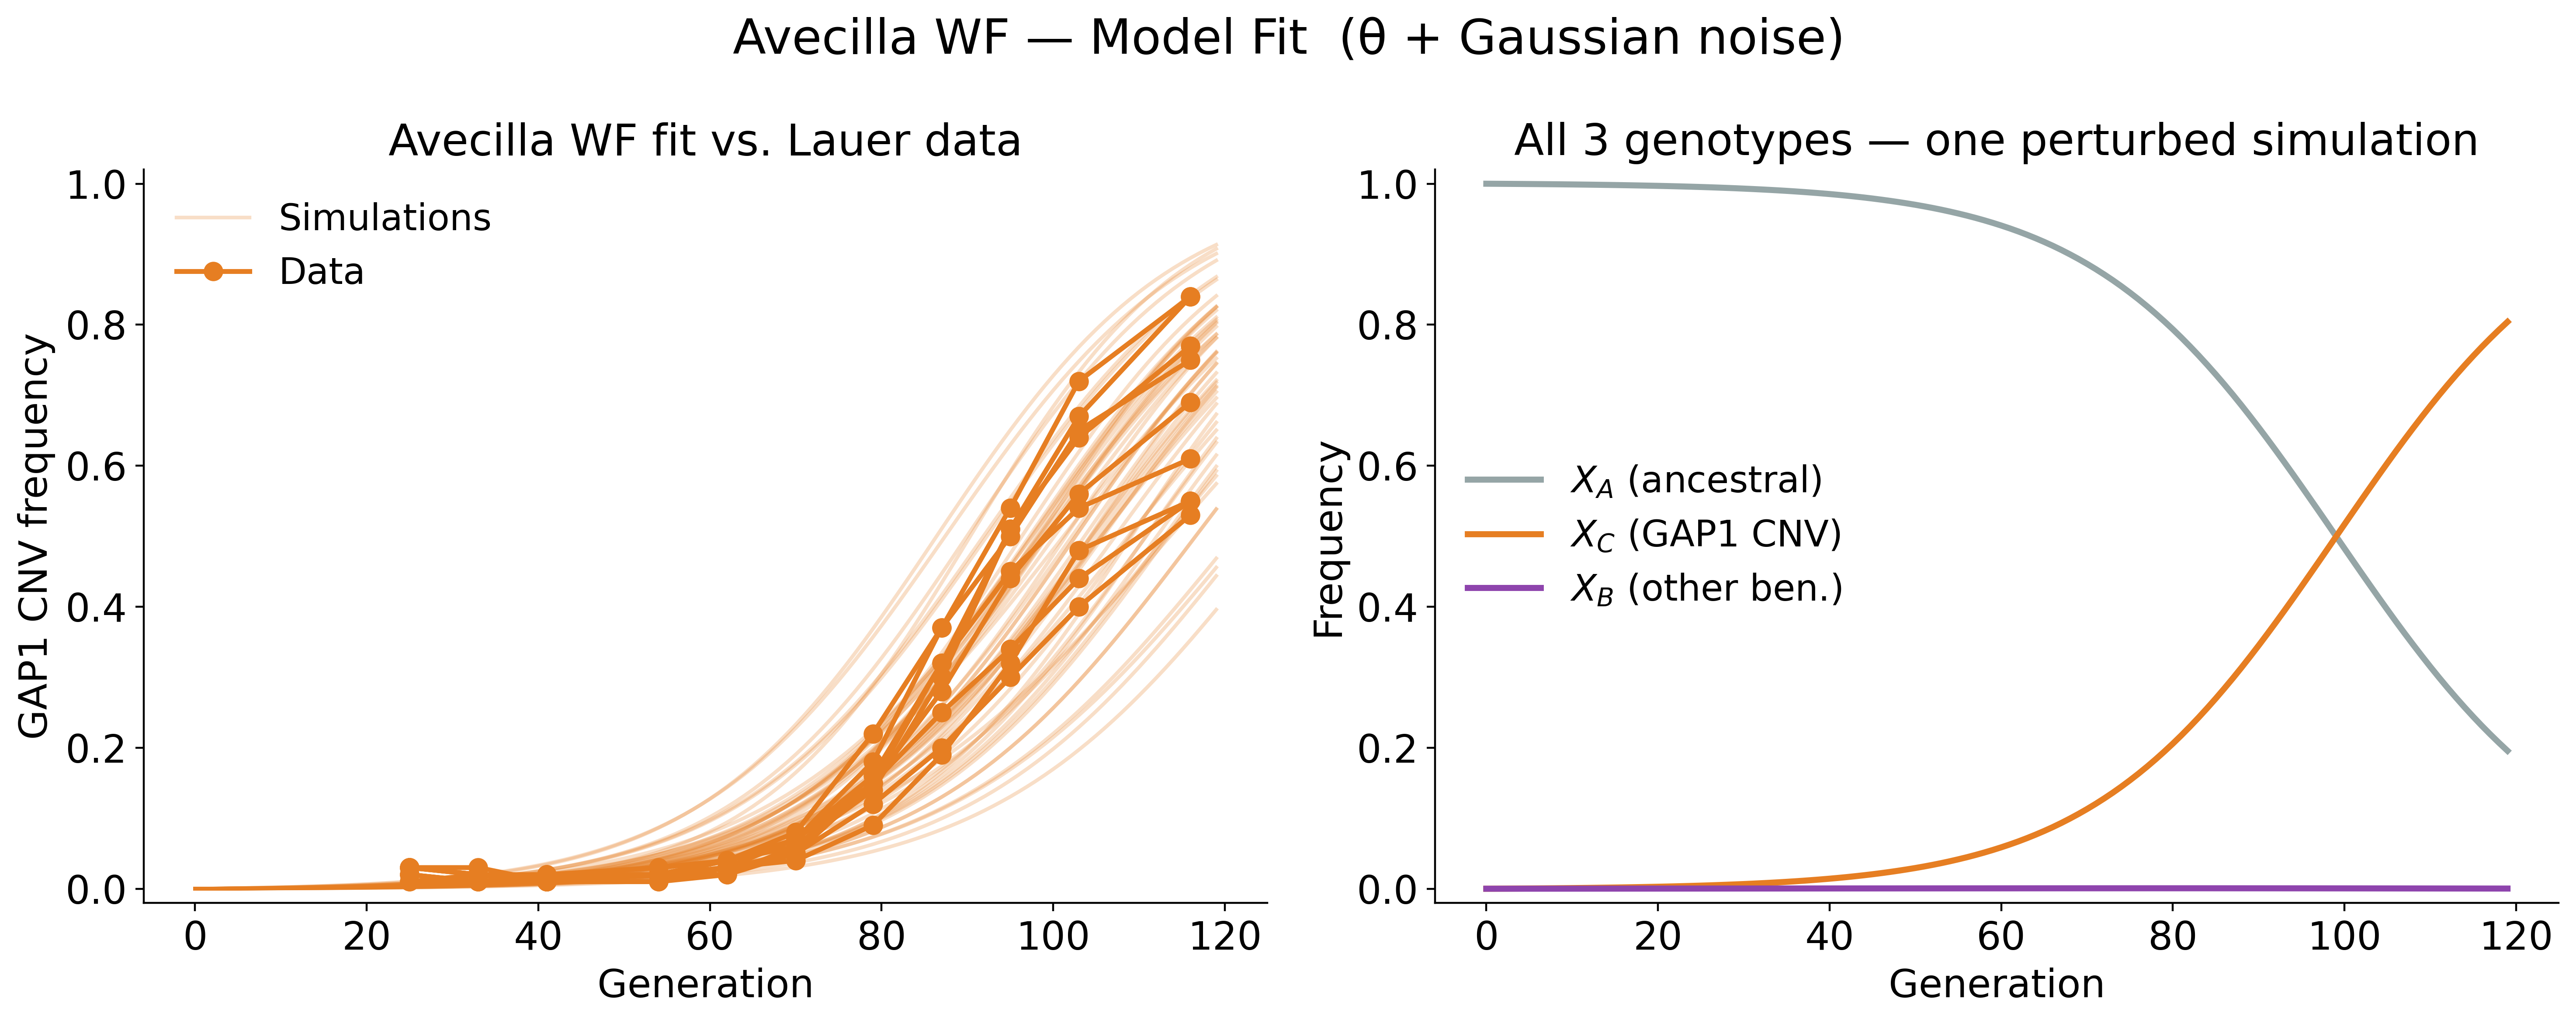
\includegraphics[width=\linewidth]{fig_avecilla_wf_fit.png}
  \caption{\textbf{Chemostat WF model fit to the Avecilla et al.\ dataset.}
  \emph{Left:} Observed CNV frequencies for nine chemostat replicate
  populations (orange dots) overlaid with simulated trajectories drawn from
  $\hat\btheta + \text{Gaussian noise}$ (light orange lines).
  \emph{Right:} A single forward simulation showing all three genotype
  frequencies ($X_A$ ancestral, $X_C$ GAP1 CNV, $X_B$ other beneficial
  mutation) over 120 generations.
  The simulation reproduces the characteristic S-shaped CNV sweep while
  keeping $X_B$ near zero, consistent with the low estimated $\delta_B$.
  (Generated by \texttt{evolution\_simulators.ipynb}.)}
  \label{fig:avecilla_wf_fit}
\end{figure}

\subsection{CNV dynamics in batch evolution (Chuong et al.\ 2025)}
\label{sec:chuong}

\subsubsection{System and data}

\citet{chuong2025template} evolved \emph{S. cerevisiae} in nitrogen-limited
serial batch culture, creating two sets of replicate lines:
LTRΔ~(7 replicates, the \emph{LTR} retrotransposon deletion background)
and ALLΔ~(8 replicates, additional deletions).
CNV frequency was tracked at 12 time points (generations 8--116) using a
locus-specific fluorescent reporter.

\subsubsection{Motivating the four-genotype model}

A natural first approach is to apply the Avecilla et al.\ three-genotype
chemostat model directly to the batch-evolution LTRΔ data.
Figure~\ref{fig:chuong_model_comparison}a shows that this produces a
systematic mismatch: simulated trajectories rise too steeply and reach
fixation too early compared with the data.
The discrepancy arises because the chemostat model does not account for
the higher effective drift and the pre-existing
CNV\textsuperscript{$-$} pool that is present in batch culture.
This motivates the four-genotype model of \citet{chuong2025template},
whose fit to the same LTRΔ data is shown in Figure~\ref{fig:chuong_model_comparison}b.
The four-genotype model correctly reproduces the plateau-and-spread
dynamics seen in the data.

\begin{figure}[ht]
  \centering
  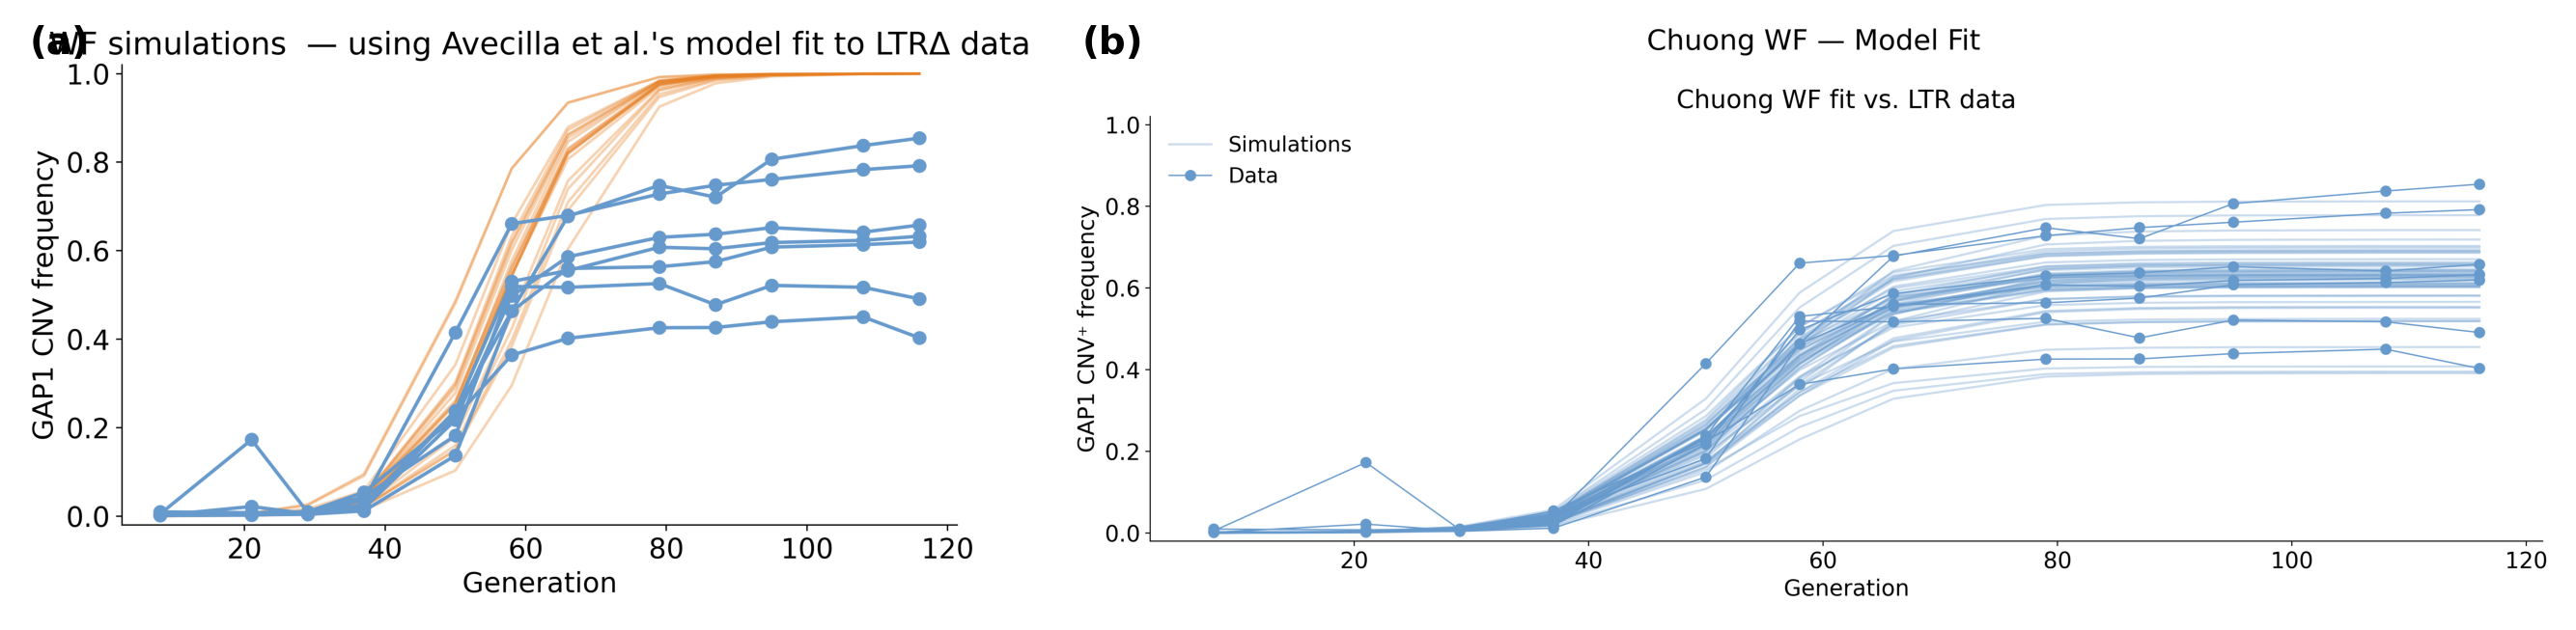
\includegraphics[width=\linewidth]{fig_chuong_comparison.png}
  \caption{\textbf{Model comparison for LTRΔ batch evolution data.}
  (a)~Applying the Avecilla et al.\ three-genotype chemostat model to the
  LTRΔ batch evolution data produces a systematic mismatch: simulated
  trajectories (orange) rise too steeply and saturate too early compared
  with the observed CNV frequencies (blue dots), because the chemostat
  model does not capture batch-culture drift dynamics.
  (b)~The four-genotype batch model of \citet{chuong2025template} fits the
  same LTRΔ data accurately (simulations in light blue).
  The model correctly reproduces the variable onset times and the plateau
  dynamics seen across replicates.
  (Generated by \texttt{evolution\_simulators.ipynb} and
  \texttt{align\_figures.ipynb}.)}
  \label{fig:chuong_model_comparison}
\end{figure}

\subsubsection{Simulator and prior}

We use the four-genotype batch WF model
(Section~\ref{sec:cnv_models}, Figure~\ref{fig:model_schematics}b) with
$N = 10^7$.
Parameters and prior ranges:
$\log s \sim \mathcal{U}(\log 0.01, \log 1)$,
$\log \delta \sim \mathcal{U}(-7, -2)$,
$\log \phi \sim \mathcal{U}(-8, -2)$.
We train the NPE on 30,000 prior samples with added Gaussian measurement
noise ($\sigma = 0.02$).

\subsubsection{Collective posterior and posterior predictive check}

Figure~\ref{fig:collective_alldelta} shows individual NPE posteriors for
each of the 8 ALLΔ replicates alongside the collective posterior computed
via Equation~(\ref{eq:collective_log}).
The collective posterior is substantially narrower than any individual
replicate posterior, providing a precise joint estimate of $(s, \delta, \phi)$
for the ALLΔ genetic background.

\begin{figure}[ht]
  \centering
  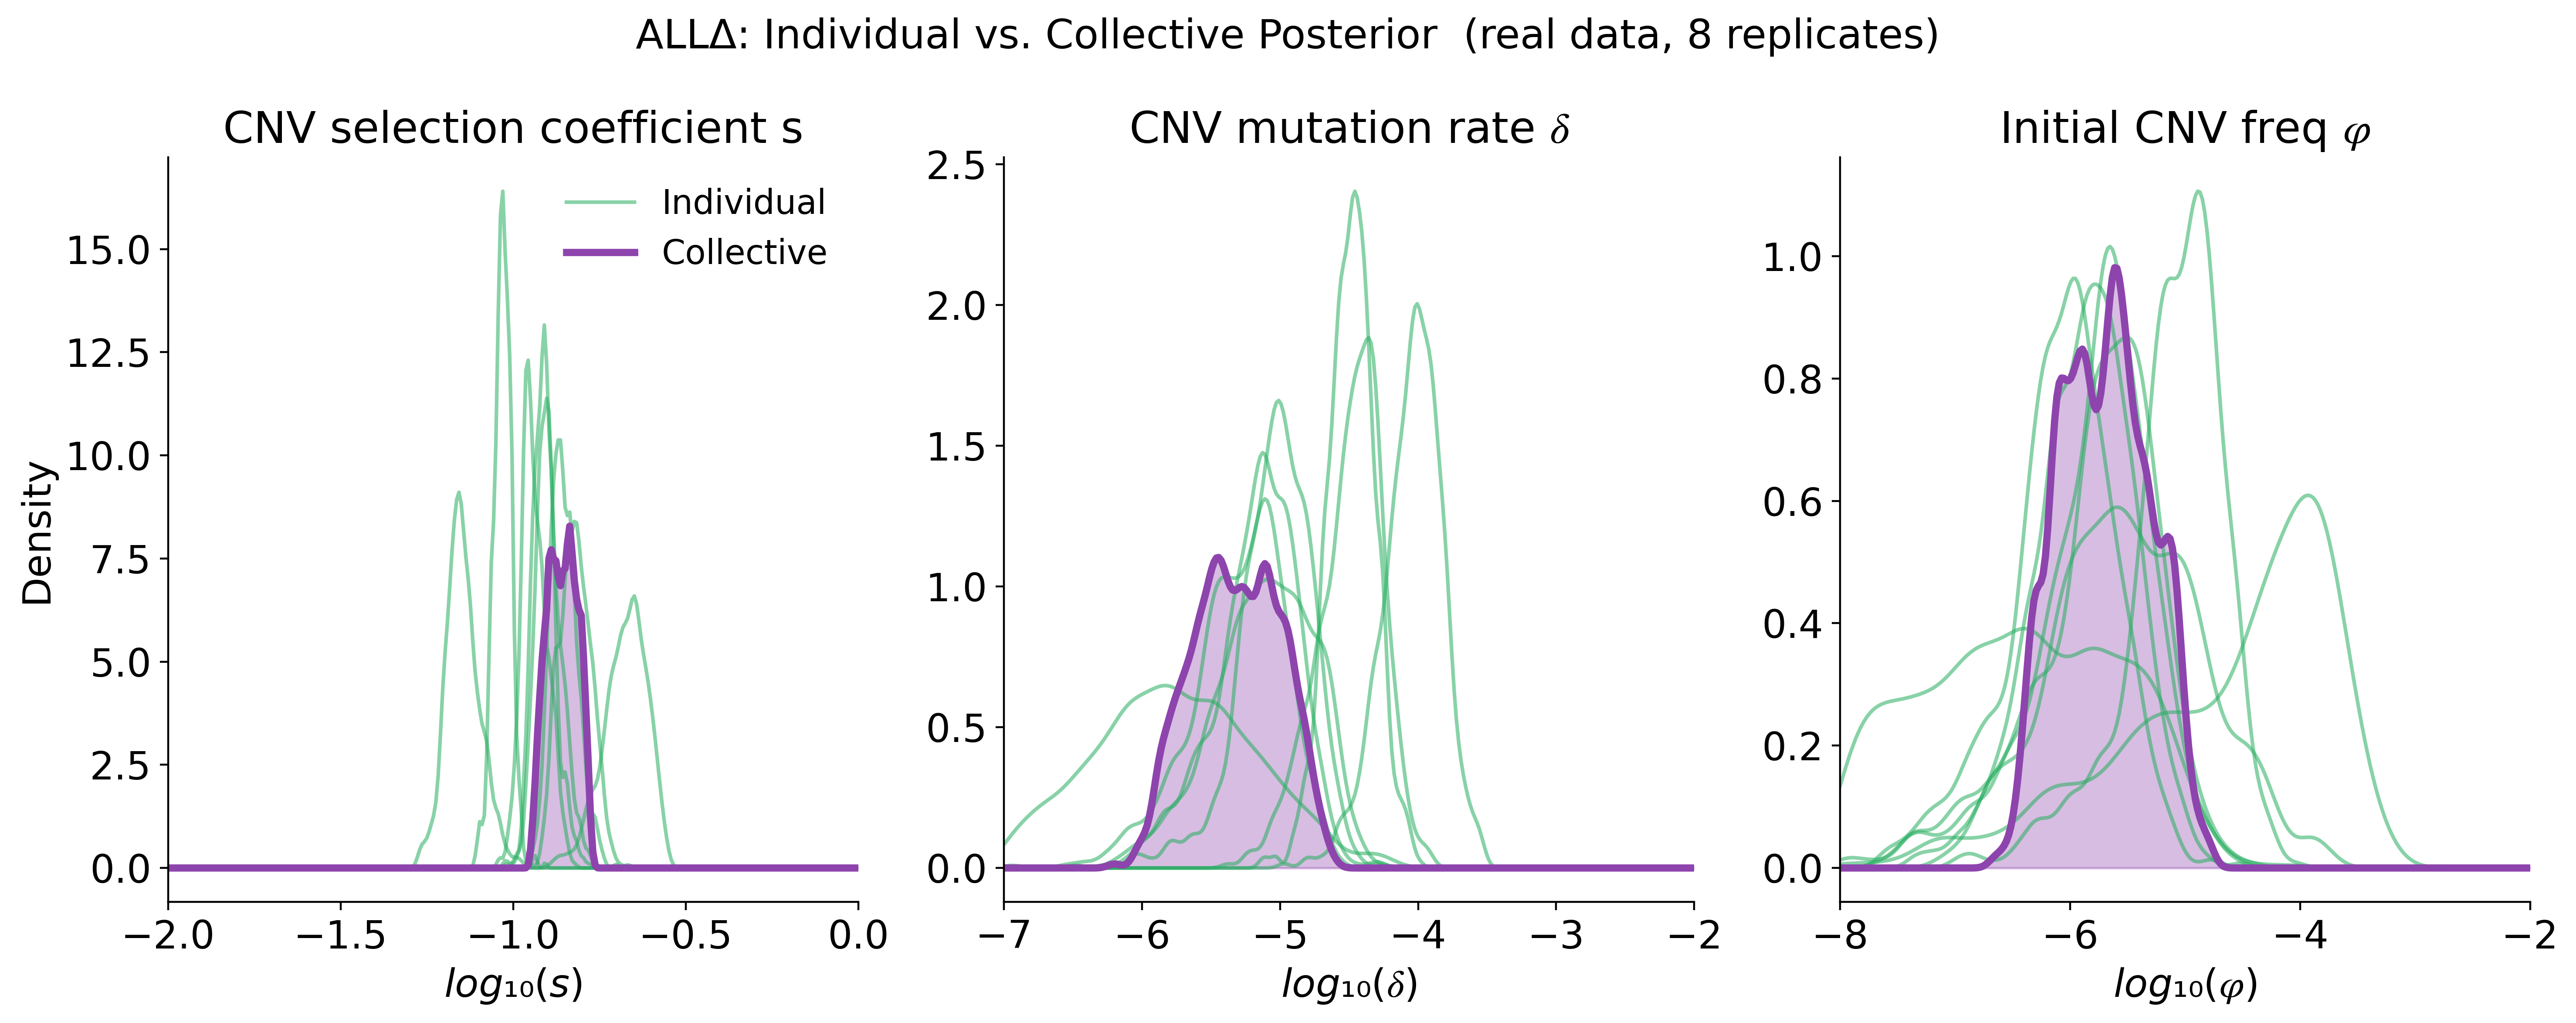
\includegraphics[width=\linewidth]{fig_collective_alldelta.png}
  \caption{\textbf{Individual and collective posteriors for the ALLΔ
  experimental lines} \citep{chuong2025template}.
  Marginal posterior densities for $\log_{10} s$, $\log_{10}\delta$, and
  $\log_{10}\varphi$ across all 8 ALLΔ replicates.
  Individual NPE posteriors (green) are broad and vary between replicates
  owing to evolutionary stochasticity.
  The collective posterior (purple), computed via
  Equation~(\ref{eq:collective_log}), integrates evidence from all
  replicates and yields a substantially tighter estimate.
  (Generated by \texttt{SBI\_tutorial.ipynb}.)}
  \label{fig:collective_alldelta}
\end{figure}

To verify model adequacy, we sample 500 parameter vectors from the
collective posterior and simulate 500 new trajectories.
Figure~\ref{fig:ppc_alldelta} shows that these posterior predictive
trajectories closely envelope the observed ALLΔ data, confirming that the
four-genotype model is well specified for this system.

\begin{figure}[ht]
  \centering
  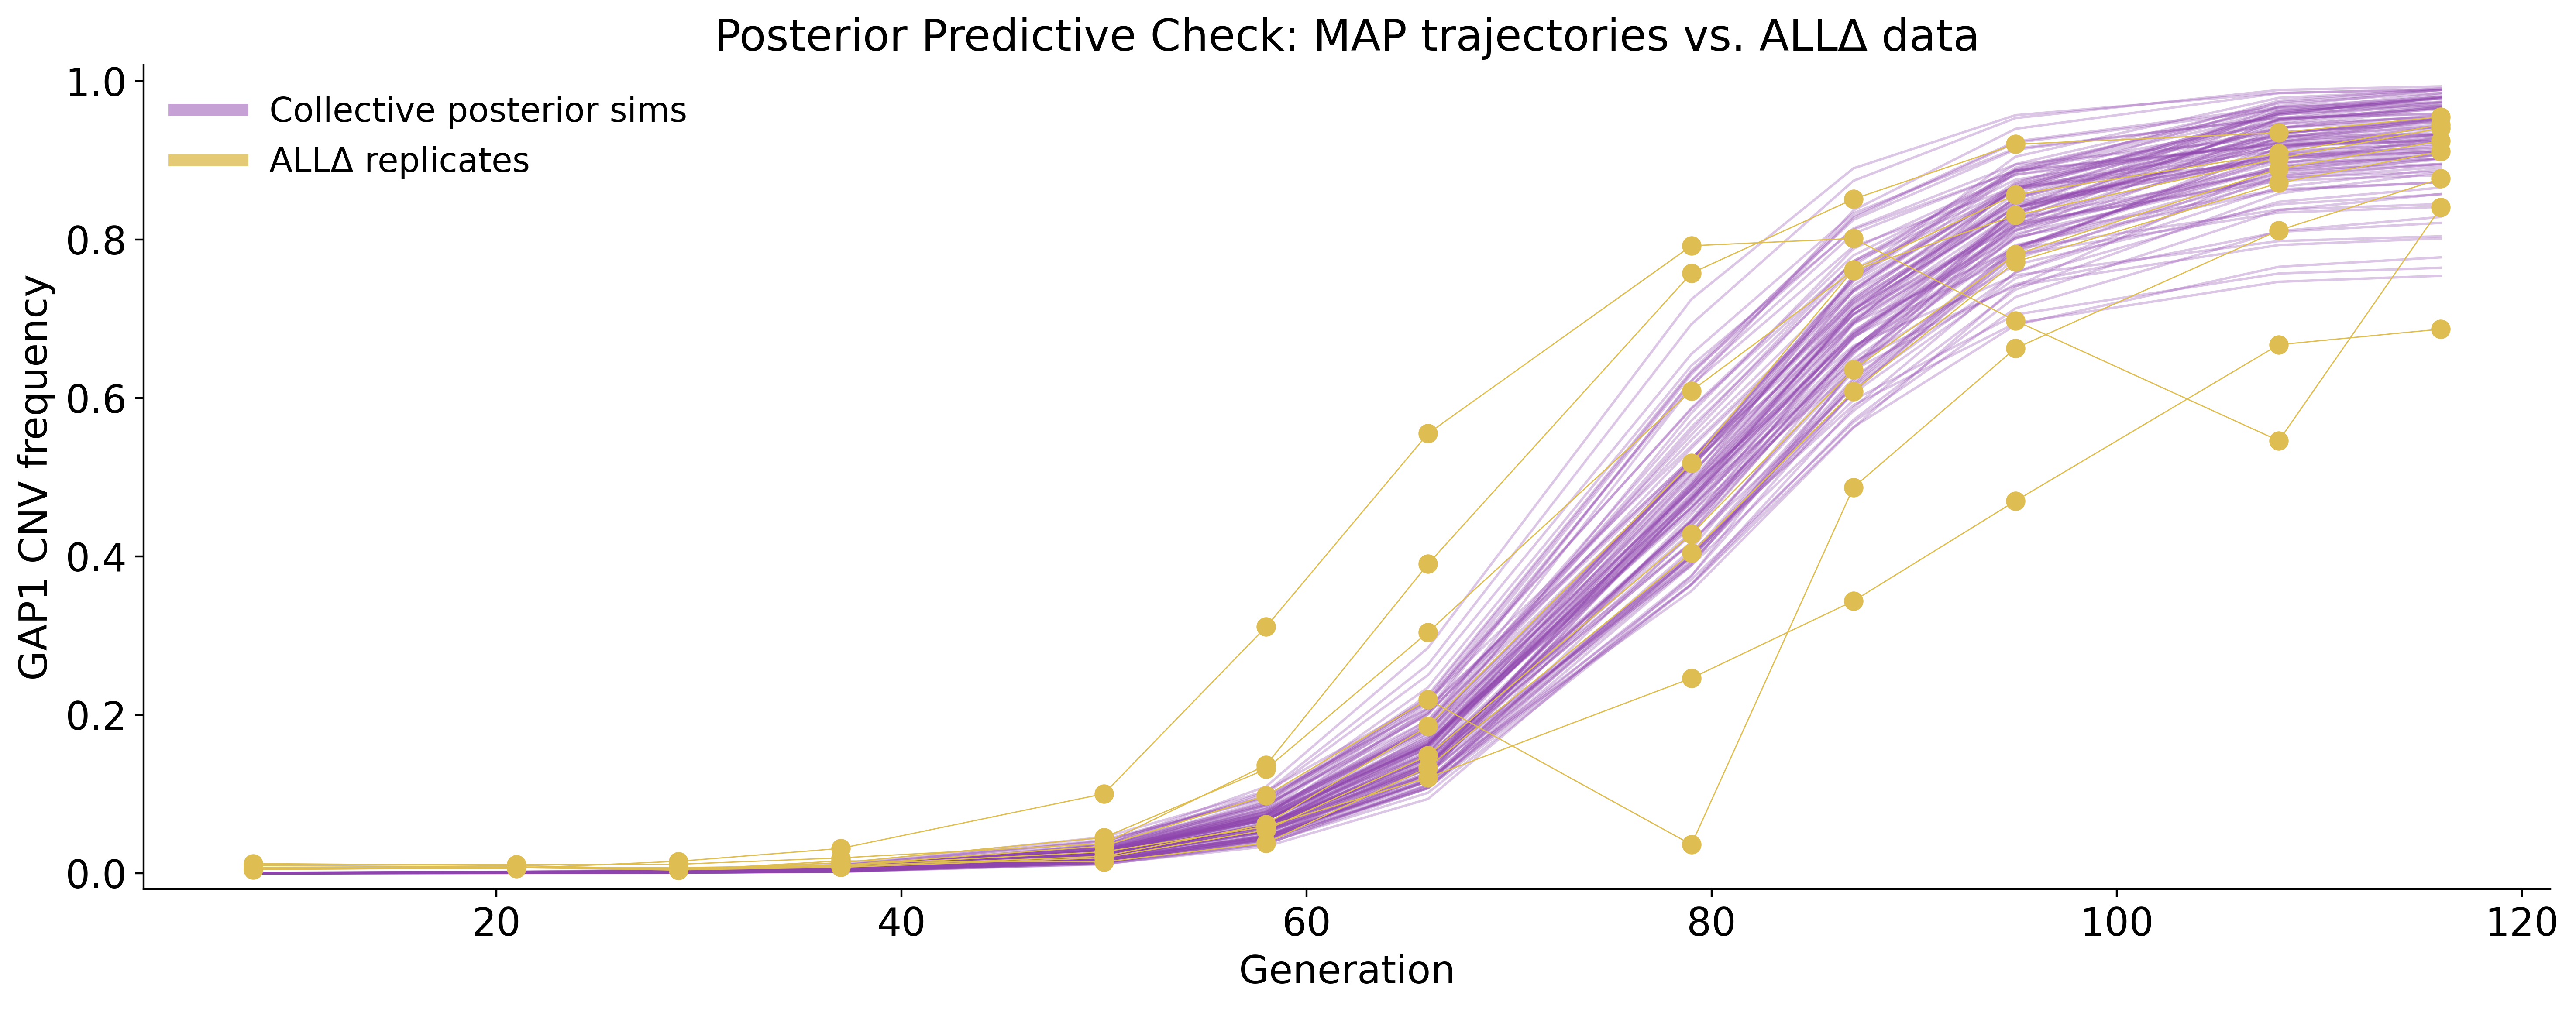
\includegraphics[width=\linewidth]{fig_ppc_alldelta.png}
  \caption{\textbf{Posterior predictive check for the ALLΔ lines.}
  Purple lines show 500 CNV frequency trajectories simulated from samples
  drawn from the ALLΔ collective posterior; yellow lines with dots show the
  8 observed ALLΔ replicate trajectories \citep{chuong2025template}.
  The simulated trajectories accurately envelope the timing and magnitude
  of the observed CNV sweeps, confirming that the four-genotype batch model
  is well specified.
  (Generated by \texttt{SBI\_tutorial.ipynb}.)}
  \label{fig:ppc_alldelta}
\end{figure}

\subsection{CNV reversion upon removal of selection (De et al.\ 2025)}
\label{sec:de}

\subsubsection{System and data}

\citet{de2025segmental} investigated the fate of \emph{GAP1} and \emph{MEP2}
CNVs when populations are returned to nutrient-replete conditions.
Fluorescent reporters tracked CNV frequency decline across 15 lineages for
110--220 generations of serial batch culture.
The study found that segmental amplifications are remarkably stable (only one
of 11 segmental-CNV strains reverted), whereas aneuploid lineages reverted
rapidly.

\subsubsection{Simulator, prior, and results}

We use the two-genotype reversion WF model
(Section~\ref{sec:cnv_models}, Figure~\ref{fig:model_schematics}c) with
$N = 1.9\times10^6$.
Parameters:
$\log s \sim \mathcal{U}(-3, 0)$ (negative selection acting on the CNV),
$\log m \sim \mathcal{U}(-5, -3)$ (reversion rate),
$\log p_0 \sim \mathcal{U}(-4, 0)$ (initial CNV frequency).
Two separate inferences are performed for the \emph{GAP1} and \emph{MEP2}
loci (Figure~\ref{fig:de_wf_fit}).
NPE inference recovers reversion rates in the range
$\hat m \approx 10^{-5}$--$10^{-3}$ for aneuploid lineages, consistent with
the high reversion rates previously estimated for whole-chromosome aneuploidy.
Segmental amplifications that did not revert are consistent with
$\hat m < 10^{-5}$ \citep{de2025segmental}.

\begin{figure}[ht]
  \centering
  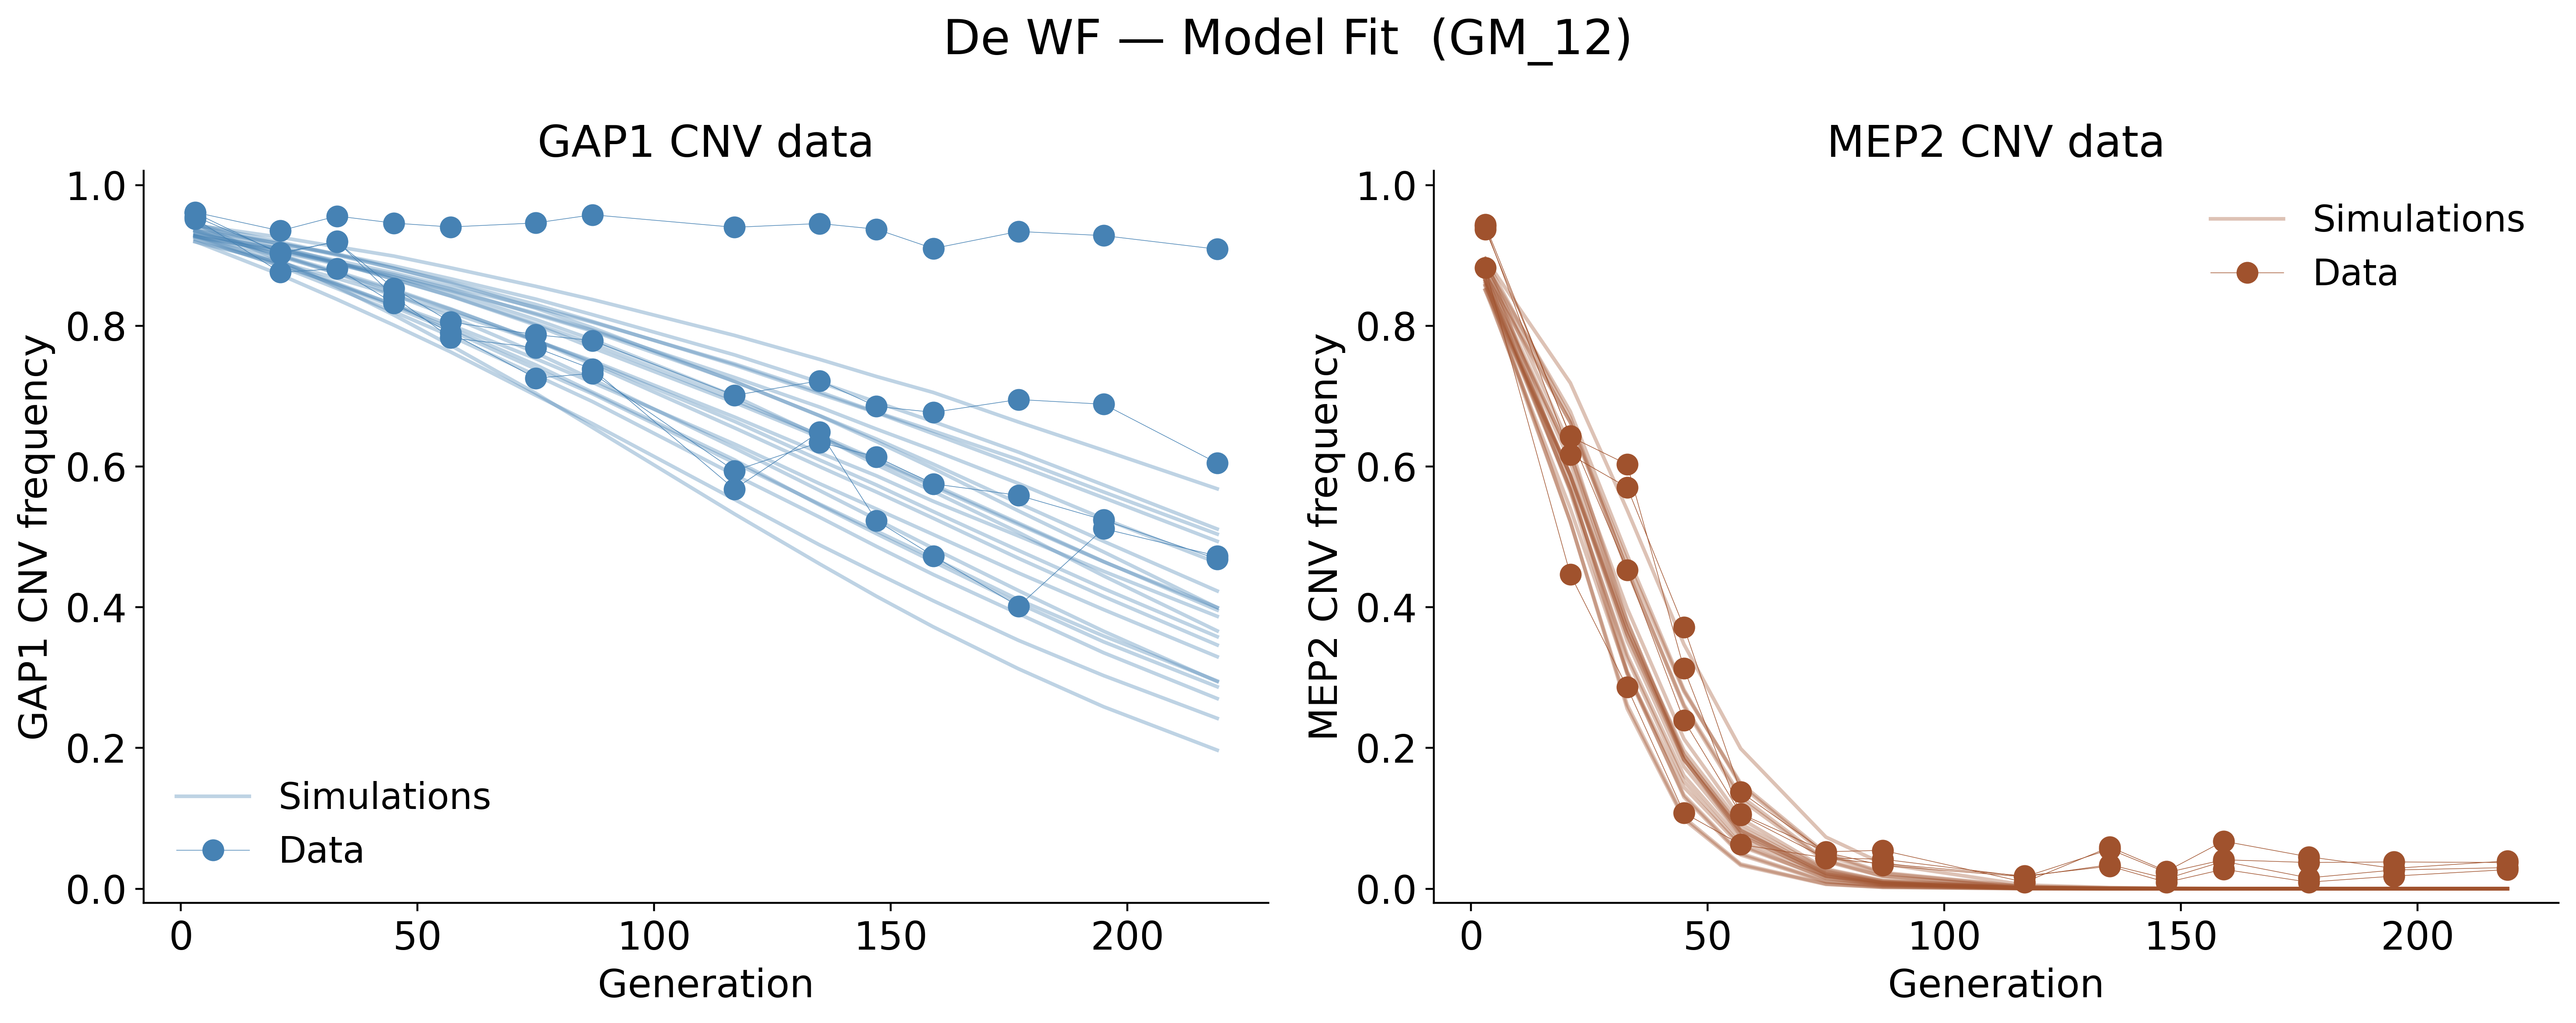
\includegraphics[width=\linewidth]{fig_de_wf_fit.png}
  \caption{\textbf{Two-genotype reversion model fit to the De et al.\ dataset.}
  Observed CNV frequencies (dots) and simulated trajectories
  (lines, $\hat\btheta + \text{Gaussian noise}$) for \emph{GAP1} CNV
  lineages (\emph{left}, blue) and \emph{MEP2} CNV lineages (\emph{right},
  brown) upon transfer to nutrient-replete conditions.
  The \emph{MEP2} locus shows faster CNV loss, reflected in a higher inferred
  reversion rate $\hat m$.
  (Generated by \texttt{evolution\_simulators.ipynb}.)}
  \label{fig:de_wf_fit}
\end{figure}

\subsection{Aneuploidy stability dynamics (Zhou et al., in prep.)}
\label{sec:zhou}

\subsubsection{System and data}

Whole-chromosome aneuploidy introduces a large-scale perturbation to gene
dosage balance.
In this system (Figure~\ref{fig:model_schematics}d), trisomic yeast are propagated
in nutrient-rich serial dilution for up to ten passages.
Three genotype frequencies---trisomic, diploid revertant, and LOH---are
simultaneously tracked using dual fluorescent reporters across $\sim 12$
replicate populations and 6 time points.

\subsubsection{Simulator, prior, and results}

We use the three-genotype aneuploidy WF model
(Section~\ref{sec:aneuploidy}) with $N_\mathrm{eff} = 10^5$.
Parameters:
$\log\mu_\mathrm{tri} \sim \mathcal{U}(-5, -1)$,
$\log\mu_\mathrm{loh} \sim \mathcal{U}(-5, -1)$,
$w_\mathrm{tri} \in (0.5, 1.2)$,
$w_\mathrm{loh} \in (0.5, 1.2)$.
Because fitness measurements for trisomic strains are available from
independent assays, $w_\mathrm{tri}$ can optionally be fixed, reducing the
inference problem to three parameters.
Figure~\ref{fig:zhou_wf_fit} shows the model fit for the Chr5 CNV GFP
reporter lines.
The simulator reproduces the characteristic rapid decline of the trisomic
population alongside a complementary rise in diploid revertants, with
the LOH population remaining at low frequency.
Full results are presented in Zhou et al.\ (in prep.).

\begin{figure}[ht]
  \centering
  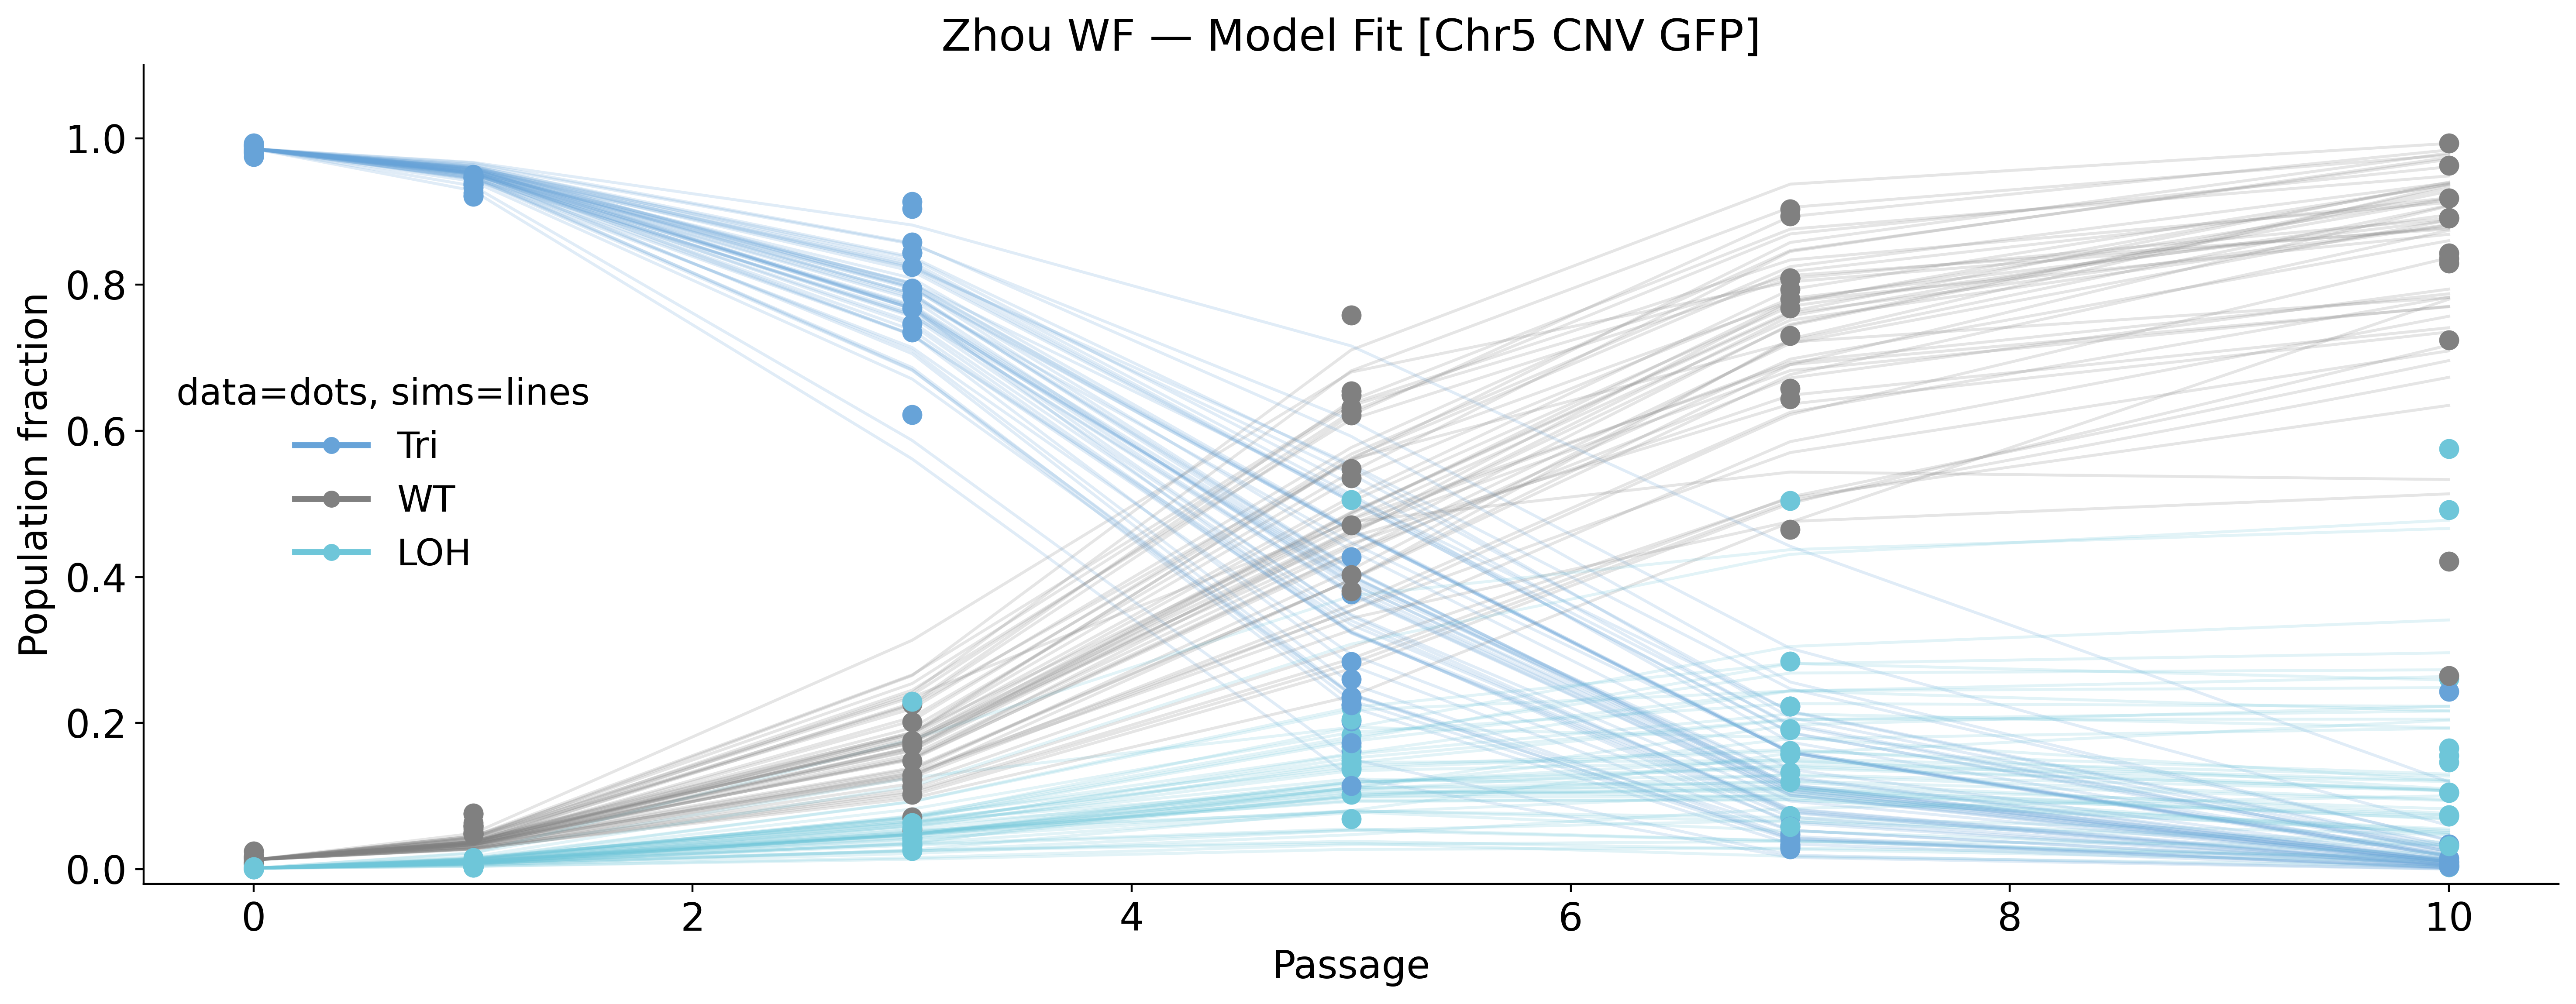
\includegraphics[width=\linewidth]{fig_zhou_wf_fit.png}
  \caption{\textbf{Three-genotype aneuploidy model fit to Chr5 CNV GFP data}
  (Zhou et al., in prep.).
  Population fractions of trisomic (Tri, blue), diploid revertant (WT,
  grey), and LOH (cyan) cells are shown across ten passages.
  Dots represent experimental observations from multiple replicate
  populations; lines show WF simulations from
  $\hat\btheta + \text{Gaussian noise}$.
  The model captures the rapid trisomic decline and the rise of both
  diploid and LOH subpopulations.
  (Generated by \texttt{evolution\_simulators.ipynb}.)}
  \label{fig:zhou_wf_fit}
\end{figure}

% =============================================================================
\section{Discussion}
\label{sec:discussion}
% =============================================================================

\subsection{Implications for reliable SBI}

The choice between ABC and neural SBI depends primarily on three factors:
simulation cost, data dimensionality, and the need for amortisation.
When simulations are cheap (milliseconds) and $T \lesssim 20$, NPE with a
single round of 30,000 simulations strikes an excellent balance between
accuracy and computational cost.
ABC remains useful for rapid prototyping before committing to neural
training, or when the simulator is stochastic in a way that makes the
loss landscape noisy.
For high-dimensional summary statistics or structured priors, NLE and NRE
provide complementary tools.

The simulator itself should be chosen to balance biological realism against
computational tractability.
We showed that a simple WF model with 3--4 genotypes suffices for CNV
dynamics in both chemostat and batch culture settings, and that the ODE
chemostat model produces nearly identical posteriors while being slower to
simulate (Figure~\ref{fig:ode_vs_wf}).
We also showed that applying the wrong model to a dataset---even one from a
closely related experimental system---produces a visible mismatch
(Figure~\ref{fig:chuong_model_comparison}), demonstrating that model
selection is a necessary step before inference.
More complex models (e.g., explicit spatial structure, fluctuating
environments) can in principle be embedded in the same SBI framework, as
long as a fast forward simulation is available.

Our broader conclusion is that \emph{reliable} SBI requires more than a good
neural density estimator.
It requires defensible prior choices, explicit model checking, and a
recognition that repeated neural training runs may themselves be a source of
uncertainty.
These observations motivate the use of ensemble estimators and
posterior-predictive checks as routine parts of the inference workflow rather
than optional add-ons.

\subsection{The collective posterior in practice}

The collective posterior (\ref{eq:collective_log}) is the statistically
correct way to combine evidence from independent replicates.
It achieves the expected $r^{-1/2}$ narrowing
(Figure~\ref{fig:collective_synthetic}), whereas a naive posterior average
shows no narrowing as $r\to\infty$.
In practice, outlier replicates---where an atypical mutation drives the
trajectory---can bias the product estimator.
The robust variant of \citet{bennun2026collective} handles this automatically
and should be preferred when outlier replicates are suspected.

A subtle but important point is that replicates are only truly ``independent''
if they share no genetic material.
In many experimental designs, replicate populations are founded from the same
ancestor, so the initial genotype state is correlated.
Accounting for this correlation may require a hierarchical model in which
replicate-specific parameters (e.g., initial frequency $\phi_i$) are drawn
from a shared hyper-prior rather than treated as independent.
This extension is straightforward within the NPE framework: one simply trains
the neural network to condition on the replicate-level observable.

\subsection{Limitations and future directions}

Several limitations of the current framework are worth noting.
First, the WF model assumes a single, well-mixed population.
Real chemostat and batch culture populations may experience spatial gradients,
clonal interference, or episodic bottlenecks that are not captured by the
basic model.
Second, observation noise is modelled as additive Gaussian, which is a
convenient approximation but may not capture the full noise structure of flow
cytometry data.
Third, the collective posterior assumes that all replicates share the same
$\btheta$; in practice, there may be biologically meaningful between-replicate
parameter variation that a single shared posterior cannot capture.

Future work could address these limitations by (i) developing multi-level
hierarchical NPE that explicitly models between-replicate variation,
(ii) incorporating richer noise models trained from calibration experiments,
and (iii) extending the simulator to include clonal interference or
spatially structured populations.
The general framework---forward simulator, NPE training, collective
posterior---is modular and can accommodate each of these extensions with
minimal changes to the inference code.

% =============================================================================
\section*{Code Availability}
% =============================================================================

All code is available in the accompanying Jupyter notebooks.
\texttt{SBI\_tutorial.ipynb} covers the complete inference pipeline for the
Chuong et al.\ ALLΔ system, from prior specification through collective
posterior sampling and posterior predictive check.
\texttt{evolution\_simulators.ipynb} demonstrates all five simulators and
their application to real experimental data.
The \texttt{CollectivePosterior} class is implemented in
\texttt{collective\_posterior.py}.
Notebooks are designed to be run sequentially and include detailed inline
comments.
Dependencies: \texttt{sbi} $\ge$ 0.22 \citep{tejero2020sbi}, PyTorch,
NumPy, SciPy, and Matplotlib.

% =============================================================================
\section*{Acknowledgements}
% =============================================================================

[Acknowledgements placeholder]

% =============================================================================
\bibliographystyle{plainnat}
\bibliography{references}
% =============================================================================

\end{document}
